\documentclass[a4paper, 16pt, oneside]{Thesis}

\usepackage{lmodern}
\usepackage{multicol}
\usepackage{pdfpages}


\usepackage{amssymb,amsmath}

\usepackage{minted}

\usepackage{dirtytalk}

\usepackage{amsthm}
%\newtheorem{definition}{Definition}
\newtheorem{observation}{Observation}

\usepackage[nameinlink]{cleveref}    

\usepackage{float}

\usepackage{enumitem}


\newminted{text}{fontsize=10pt}

\newfloat{code}{h}{smp}
\floatname{code}{Code sample}

\crefname{code}{code sample}{code samples}
\Crefname{code}{Code sample}{Code samples}


% use upquote if available, for straight quotes in verbatim environments
\IfFileExists{upquote.sty}{\usepackage{upquote}}{}
% use microtype if available
\IfFileExists{microtype.sty}{%
\usepackage{microtype}
\UseMicrotypeSet[protrusion]{basicmath} % disable protrusion for tt fonts
}{}
%\usepackage{geometry}
%\geometry{%
%letterpaper, % a4paper
%left=   40 mm,
%right=  40 mm,
%top=    15 mm,
%bottom= 20 mm,
%}


\hypersetup{breaklinks=true,
            bookmarks=true,
            pdfauthor={Harm Delva},
            pdftitle={Static Analysis of Dynamic Languages},
            colorlinks=false,
            citecolor=blue,
            urlcolor=blue,
            linkcolor=magenta,
            pdfborder={0 0 0}}
\urlstyle{same}  % don't use monospace font for urls

\setlength{\parindent}{0pt}
\setlength{\parskip}{6pt plus 2pt minus 1pt}
\setlength{\emergencystretch}{3em}  % prevent overfull lines
\providecommand{\tightlist}{%
  \setlength{\itemsep}{0pt}\setlength{\parskip}{0pt}}

\title{Static Analysis of Dynamic Languages}
\author{Harm Delva}
\date{}

% Redefines (sub)paragraphs to behave more like sections
\ifx\paragraph\undefined\else
\let\oldparagraph\paragraph
\renewcommand{\paragraph}[1]{\oldparagraph{#1}\mbox{}}
\fi
\ifx\subparagraph\undefined\else
\let\oldsubparagraph\subparagraph
\renewcommand{\subparagraph}[1]{\oldsubparagraph{#1}\mbox{}}
\fi

\usepackage[noend]{algpseudocode}
\usepackage{algorithm}
\usepackage{cleveref}

\usepackage{amsmath} % nice math symbols     

\usepackage{tikz}

\usetikzlibrary{matrix} % for block alignment
\usetikzlibrary{arrows} % for arrow heads
\usetikzlibrary{calc} % for manimulation of coordinates

% TikZ styles for drawing
\tikzstyle{block} = [draw,rectangle,thick,minimum height=2em,minimum width=2em]
\tikzstyle{sum} = [draw,circle,inner sep=0mm,minimum size=2mm]
\tikzstyle{connector} = [->,thick]
\tikzstyle{line} = [thick]
\tikzstyle{branch} = [circle,inner sep=0pt,minimum size=1mm,fill=black,draw=black]
\tikzstyle{guide} = []
\tikzstyle{snakeline} = [connector, decorate, decoration={pre length=0.2cm,
                         post length=0.2cm, snake, amplitude=.4mm,
                         segment length=2mm},thick, magenta, ->]

\renewcommand{\vec}[1]{\ensuremath{\boldsymbol{#1}}} % bold vectors
\def \myneq {\skew{-2}\not =} % \neq alone skews the dash

\usepackage{minted}
\usemintedstyle{manni}
\usepackage{mathtools}
\usetikzlibrary{positioning, calc}
\usepackage{subcaption}
\usepackage[compatibility=false]{caption}
\usepackage{graphicx}

\usepackage{tcolorbox}
\tcbuselibrary{minted}
\tcbuselibrary{skins}

\definecolor{bg}{HTML}{F0F3F3}

\usepackage{letltxmacro}
\LetLtxMacro{\oldhypertarget}{\hypertarget}
\renewcommand{\hypertarget}[2]{\leavevmode\oldhypertarget{#1}{#2}}

\newcommand{\nocontentsline}[3]{}
\newcommand{\tocless}[2]{\bgroup\let\addcontentsline=\nocontentsline#1{#2}\egroup}

\newenvironment{Figure}
  {\par\medskip\noindent\minipage{\linewidth}}
  {\endminipage\par\medskip}

\begin{document}

\title  {Static Analysis of Dynamic Languages}
\authors  {\texorpdfstring
            {\href{harm.delva@gmail.com}{Harm Delva}}
            {Harm Delva}
            }
\date       {\today}
\subject    {}
\keywords   {}

\maketitle

\cleardoublepage
\thispagestyle{empty}
\begin{center}{\huge\bf Preface}\end{center}
    {\vfill\null}
      Writing this dissertation wouldn't have been possible without some help -- so some special thanks are in order. I'd like to thank the following people, in no particular order:

      \begin{itemize}[label={}]
        \item Prof. Dr. Peter Dawyndt for his guidance and insights while writing this dissertation. 
        \item My parents, friends, and other family for the moral support over the years. 
        \item Everyone involved at Ghent University, fellow students and professors alike, who have kept me motivated and curious. 
        \item My girlfriend --  who graciously donated her submissions to be used as part of this dissertation -- for everything.  
      \end{itemize}
 
    {\vfill\null}

\setstretch{1}
            
\pagenumbering{gobble}

% The Preface page, for thanking everyone.
%\preface{
%Fuck all of you.
%}
%\clearpage

%\abstracts{

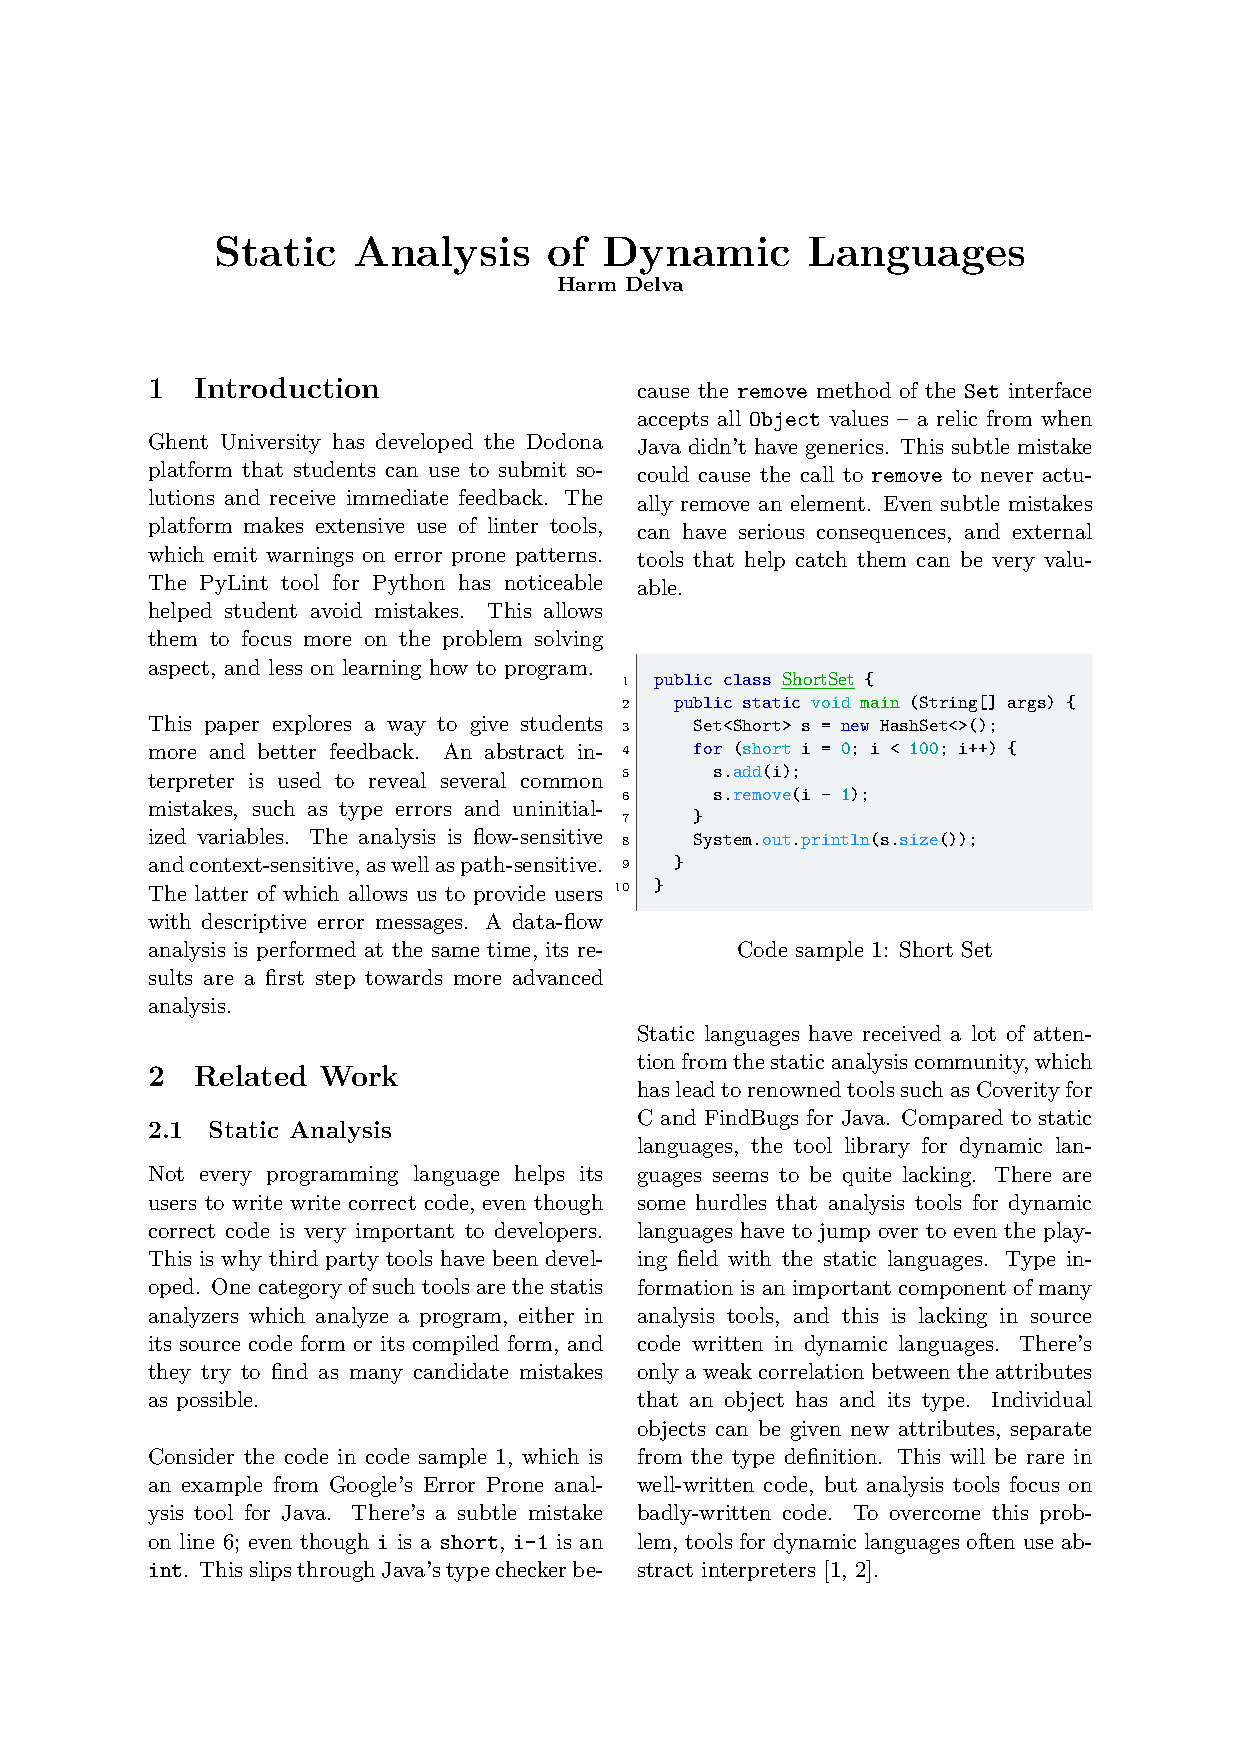
\includepdf[pages={-}, fitpaper=true, offset=75 0]{abstract.pdf}


\tableofcontents

\hypersetup{
    colorlinks = true,
}

\renewcommand{\thesection}{\thechapter.\arabic{section}} 
\renewcommand{\thesubsection}{\thesection.\arabic{subsection}}

\mainmatter
\setstretch{1.3}
\pagenumbering{arabic}

\chapter{Context}\label{context}

Ghent University has developed the Dodona platform\footnote{\url{dodona.ugent.be}
  -- accessed 31 May 2017} that students can use to submit solutions and
receive immediate feedback. This feedback is in large part done through
unit testing which lets the students know whether or not their solution
is correct, but it doesn't really help them forward if it's not. To
remedy this, a visual debugger is available which students can use to
step through their program. Unfortunately it is limited in what it can
do. More importantly, it can only let the user scroll through execution
states. If an error occurred after a couple of thousand executed
statements, this becomes a very tedious process.

There are ways to avoid the pain of debugging altogether. There are
linter tools such as JSLint and Pylint which emit warnings on error
prone patterns. The Dodona platform uses these tools as well, and relays
the warnings to the students.

The Pylint tool for Python has noticeably helped students avoid
mistakes. This in turn allowed them to focus more on the problem solving
aspect and less on learning how to program. The goal of this
dissertation is to build on top of that, giving the students even more
and even better feedback. An extensive data-flow analysis can untangle
even the worst spaghetti code, which makes it a prime starting point for
further analysis and feedback.

\chapter{Related Work}\label{related-work}

\section{Static Analysis}\label{static-analysis}

NASA's source code of the Apollo 11 Guidance Computer was recently
digitized and put on GitHub.\footnote{\url{https://github.com/chrislgarry/Apollo-11}
  -- accessed 31 May 2017} All of it was written in an assembly language
and the result worked just fine. The C programming language was
developed for the Unix operating system so the latter could run on
various CPU architectures {[}32{]}. In essence it's a pretty thin
abstraction over assembly, in the sense that it doesn't take much
pressure off of the programmers. Unix worked just fine, just like NASA's
guidance controller. One could argue that programmers don't need tools
to aid them -- they seem to know what they're doing.

As the field of computing grew, and with it the projects, it started
becoming apparent that programmers can't always rely on themselves. Even
veteran developers occasionally discover a major vulnerability in their
code -- like the Heartbleed vulnerability in OpenSSL.\footnote{\url{http://heartbleed.com/}
  -- accessed 31 May 2017} Of course everyone makes mistakes , but
critical code should avoid them at all costs. A first line of defense
against these costly mistakes is a proof of correctness. NASA's code was
reliable because they had formal proofs that the most critical parts
were correct {[}6, 14, 21{]}. Doing this is a massive amount of work,
and a proof can still be wrong. More importantly, most verification
frameworks are applied to designs and not implementations {[}34{]}.

Functional programming languages are closely related to provable
correctness, while also automating some of the checks. Notable examples
of such languages are Haskell and ML. Both have a strong theoretical
foundation and provide the programmer with a strong type system to make
it easier to reason about the code. This stands in strong contrast with
languages like C. While Haskell was made to facilitate writing correct
code {[}30{]}, C was made to be close to the metal and efficient
{[}32{]}. The C compiler doesn't help the programmer nearly as much as
the Haskell compiler. Developing correct and functional programs is
obviously paramount to any programmer, so C's priorities don't always
align with those of the developer.

That's where static analyzers come into play. They analyze a program,
either in its source code form or its compiled form, and try to find as
many candidate mistakes as possible. These mistakes are often very
subtle and rare, but even a single one can ruin someone's week. Code
sample \ref{smp:shortset} comes from Google's Error Prone GitHub
page\footnote{\url{https://github.com/google/error-prone} -- -- accessed
  31 May 2017} and is a great example of how subtle serious bugs can be.
The code seems to be just fine at first glance, the analysis in sample
\ref{smp:shortset_f} reveals a subtle flaw.

\begin{code}
  \begin{tcblisting}{listing only, 
  arc=0pt,
  outer arc=0pt, 
  boxrule=0.2pt,
  minted language=java,
  minted style=autumn,
  minted options={xleftmargin=-6pt, linenos},
  colback=bg }
public class ShortSet {
  public static void main (String[] args) {
    Set<Short> s = new HashSet<>();
    for (short i = 0; i < 100; i++) {
      s.add(i);
      s.remove(i - 1);
    }
    System.out.println(s.size());
  }
}
\end{tcblisting}
\caption{Short Set}\label{smp:shortset}
\end{code}

\begin{code}
  \begin{tcblisting}{listing only, 
  arc=0pt,
  outer arc=0pt, 
  boxrule=0.2pt,
  minted language=HTML,
  minted style=autumn,
  minted options={xleftmargin=-6pt, linenos},
  colback=bg }
error: [CollectionIncompatibleType] Argument 'i - 1' should not be 
passed to this method; its type int is not compatible with its 
collection's type argument Short
      s.remove(i - 1);
              ^
\end{tcblisting}
\caption{Analysis of code sample \ref{smp:shortset}} \label{smp:shortset_f}
\end{code}

Subtracting an \texttt{int} from a \texttt{short} results in an
\texttt{int}. In this case it won't cause an actual bug yet, because
both types use the same hashing function. But this isn't something a
developer should rely on. The JVM originally didn't support generics,
and their implementation is still a bit rough. The \texttt{remove}
method of a \texttt{List} instance accepts any \texttt{Object} instance.
This can result in calls that never actually remove anything. If that
call happens to only occur in a corner case in the \(1000^{\text{th}}\)
iteration of a loop, this can lead to some very confusing bugs.

\subsection{Popular Languages}\label{popular-languages}

Every practical programming language is Turing complete, so in theory
they should all be equal. This is a misconception that has been called
the Turing tar-pit {[}44{]}. Everything is possible in a Turing tar-pit,
but nothing of interest is easy. Programming languages where things of
interest are perceived to be easy can be considered powerful. These
languages are often the ones with lenient compilers or runtime
environments such as C, Python, Javascript, \ldots{} In other words,
languages that don't get in the way of the programmer too often. These
are also by far the most popular languages.

As illustrated in the previous section, this may not always be a good
idea as humans tend to glance over subtle details. This makes the need
for additional tools very important for any project that aims to achieve
high reliability. The alternative is long and painful debugging
sessions. At some point these languages no longer make it easy to do
things of interest.

\subsubsection{C}\label{c}

The C programming language has been one of the most popular programming
languages for a couple of decades now. Depending on who you ask, the
best thing about C is either its efficiency or its simplicity. The
latter is what gives developers the power they desire. This comes at a
cost however; with great power comes great responsibility.

Let's focus on the other main attraction of C, its efficiency. This
comes at a cost as well and it's one many people forget about. C's
\emph{raison d'être} isn't making developers feel good about themselves,
it's generating efficient code. It was created to be a thin abstraction
layer over various assembly languages that were limiting software
development at the time {[}32{]}. This has left some holes in the C
specification; for example, not all CPU architectures handle a division
by zero, so the C specification doesn't specify what to do in this case.

\paragraph{Undefined Behavior}\label{undefined-behavior}

There are a lot of things the C specification doesn't specify a behavior
for, which leads to undefined behavior. Some are well-known, such as
using freed memory. Others catch people by surprise. For example, the
GNU libc website claims that \texttt{1/0} yields \texttt{inf},\footnote{\url{http://www.gnu.org/software/libc/manual/html_node/Infinity-and-NaN.html}
  -- accessed 31 May 2017} even though the C99 specification clearly
contradicts them {[}15{]}. The C99 standard introduced the \texttt{INF}
macro, but it doesn't specify which operations should result in one.
Division by zero is still as undefined as it has always been.

Entire papers have been written on the subject of undefined behavior
{[}35, 40, 49{]}. One striking thing is how recent a lot of these papers
are. Even though the language is over 40 years old, this is still an
active field of research. Compilers are getting more advanced and with
it the optimizations they perform. Some of those optimizations rely on
the fact that the compiler is under no particular obligation when
optimizing code containing undefined behavior.

\begin{code}
  \begin{tcblisting}{listing only, 
  arc=0pt,
  outer arc=0pt, 
  boxrule=0.2pt,
  minted language=C,
  minted style=autumn,
  minted options={xleftmargin=-6pt, linenos},
  colback=bg }
if (arg2 == 0)
  ereport(ERROR, 
    errcode(ERRCODE_DIVISION_BY_ZERO),
    errmsg("division by zero"));
                    
/* No overflow is possible */
PG_RETURN_INT32((int32) arg1 / arg2);
\end{tcblisting}
\caption{Undefined Behavior}\label{smp:undef}
\end{code}

Code sample \ref{smp:undef} was part of PostgreSQL {[}35{]}. The call to
\texttt{ereport} on line 2 never returns. It does some logging before
calling \texttt{exit}. In the mind of the developer this prevents the
division by zero on line 7. Looking at the code on GitHub,\footnote{\url{https://github.com/postgres/postgres/blob/master/src/backend/utils/adt/int.c\#L847}
  -- accessed 31 May 2017} the function this sample came from indicates
that calling it will return a \texttt{Datum} struct. According to the
language specification, this function \emph{must} return a value each
time it's called. The body of the null check does not return anything,
so the compiler concludes that the rest of the function will also be
executed and division by \texttt{arg2} will always occur.

Division by zero is also undefined behavior in C, so the compiler
concludes that \texttt{arg2} won't ever be zero -- it wouldn't get used
in a division otherwise. As a result, the null check gets flagged as
dead code, and is removed entirely.

\begin{code}
  \begin{tcblisting}{listing only, 
  arc=0pt,
  outer arc=0pt, 
  boxrule=0.2pt,
  minted language=C,
  minted style=autumn,
  minted options={xleftmargin=-6pt, linenos},
  colback=bg }
if (arg2 == 0)
{
  ereport(ERROR,
      (errcode(ERRCODE_DIVISION_BY_ZERO),
       errmsg("division by zero")));

  /* ensure compiler realizes we mustn't reach the division 
  (gcc bug) */
  PG_RETURN_NULL();
}
\end{tcblisting}
\caption{Fixed Undefined Behavior}\label{smp:undef_f}
\end{code}

Code sample \ref{smp:undef_f} contains the fixed code. By adding an
explicit return (in the form a macro), the compiler leaves the null
check intact. Notice how the comment blames a ``gcc bug''. This
illustrates how even experienced developers seem to misunderstand their
language of choice.

\paragraph{Tools}\label{tools}

Not a single other programming language comes close to having as many
external tools as C (and by extension C++). Many developers heavily
depend on these tools in their usual workflow. One of the most
established toolsets are the ones in Valgrind.

Valgrind is a suite of dynamic analysis tools, the most famous of which
is Memcheck. Memory related bugs are some of the hardest to track down
because they're ultimately undefined behavior. For example, using a
memory location after freeing might not always crash the program.
There's an informal term for bugs like these: \emph{heisenbugs}.
Something might go wrong but when you try to isolate the cause
everything seems to be just fine. Especially since Address Space Layout
Randomization (ASLR) tends to be disabled during debugging but not
during normal execution.

This is where Memcheck comes into play. It analyses the program during
regular execution and keeps track of what happens to the memory. This
way it can notice memory related bugs such as use-after-free and report
them back to the developer. Unfortunately it's not a perfect solution.
There can be false positives as well as false negatives, and it is quite
incompatible with some libraries such as OpenMPI {[}45{]}.

A lot of companies rely on analysis tools to manage their large C
projects, and when there's demand in a market, the supply will follow.
There's an impressive amount of commercial analysis tools available.
Coverity is one of the most established ones.

Dawson Engler, one of Coverity's co-founders, is one of the leading
researchers in the field of static analysis. He also co-authored a great
paper in which he describes how difficult static analysis is in the real
world {[}4{]}. One particularly interesting part of the paper explains
that there's a fundamental misunderstanding of what programming
languages and compilers are. A programming language can exist as an
abstract idea or a piece of paper. While the language a program is
written in is whatever the compiler accepts. In other words, compilation
is not certification. A good first step for a static analysis tool is to
make sure that the input adheres to the specification. They go on to
pose the hypothetical question: ``Guess how receptive they {[}the
end-users{]} are to fixing code the ``official'' compiler accepted but
the tool rejected with a parse error?''

Even with a plethora of tools available, C remains an untamed beast.
Some tools like Valgrind are great at what they do but are still
limited. Other tools like Coverity seem to fight stubborn developers as
often as they fight bugs.

\subsubsection{Dynamic Languages}\label{dynamic-languages}

According to Guido Van Rossum, he designed Python because he wanted to
make a descendant of ABC that would appeal to Unix/C hackers {[}23{]}.
This is a bit worrying considering the previous section, as C is a
remarkably hard language to analyze. Javascript's situation isn't great
either. There are no namespaces, no modularization system, no classes,
no interfaces, no encapsulation, and so on. Eric Lippert, who was on the
ECMA committee during the early days of JavaScript, has a Stackoverflow
post where he discusses why Javascript is so ill-fit for static analysis
and programming in the large {[}43{]}. Even though Stackoverflow is a
dubious source for any academic work, the author's experience should
make up for it.

Both Python and JavaScript are popular languages, so one might expect
there to be a good amount of analysis tools for these languages as well.
There seem to be two classes of analysis tools available for these
languages right now: linters and type checkers. The linters are very
popular, but as a later section will discuss they focus on error prone
patterns instead of errors, and they prioritize efficiency over in-depth
analysis. Type checkers are less popular, mostly due to circumstances.

A type analysis tool for Javascript called JSure was developed in 2009,
in part because the authors felt a need for deeper analysis than what
JSLint could offer {[}16{]}. They utilize an abstract interpreter to
perform a flow- and context-sensitive analysis. Typescript was released
a few years later, which fills a similar function as JSure, but with the
researching power of Microsoft behind it. Python has a similar tool
called MyPy which takes a fundamentally different approach {[}17{]}.
Python 3.5 introduced type hints for analysis tools such as MyPy to use.
Although promising, the tool is plagued with a few limitations. For
starters, it only supports Python versions since 3.5, while the users
who stand the most to gain from it are the ones with large code bases --
which are predominantly on version 2.x for legacy reasons. On top of
that, most existing Python 3 code does not even use type hints at this
point, so stand nothing to gain from MyPy.

What these two classes of analysis tools for dynamic languages have in
common is that they're not as in-depth as the ones for static languages.
Tools like Coverity for C and Error Prone or FindBugs for Java go as far
as detecting racing conditions, while the tools for Javascript and
Python are still experimenting with type analysis. This isn't because
dynamic languages aren't important, they're used to power some of the
biggest websites {[}13, 18{]}, it's just a hard thing to do. The
following anecdotal examples illustrate why.

\clearpage

\paragraph{Classes}\label{classes}

Lots of developers are familiar with class hierarchies and like using
them, but there is one glaring difference between how static languages
and dynamic languages handle classes. In most static languages, the
class definition declares which methods and attributes are defined for
objects of that class. This isn't the case with dynamic languages.
Adding a method to an object is as simple as adding a callable object to
the class's namespace. This is bad news for static analyzers that try to
do type inferencing on dynamic languages. Consider the following bug
that occurred while I was working on the Dodona platform.

The Ruby builtin \texttt{String} class provides a \texttt{split} method
that does the same thing as in most other languages: its argument is
some separator that is used to cut the \texttt{String} object into an
array of smaller \texttt{String} objects. While writing a function that
takes a few strings as arguments, the strings had to be split on
whitespace. Calling the \texttt{split} method on one of the strings
returns the same object instead. Using \texttt{puts} on that object just
shows the same exact \texttt{String} we wanted to split, with all the
whitespace still there, weird. The documentation says that it should
work. Testing the method in a REPL (Read--eval--print loop) environment
confirms that the \texttt{split} method should indeed split the
\texttt{String}. A few confused hours later, it turned out the object
wasn't a \texttt{String} but an \texttt{Array} of \texttt{String}
objects. The Ruby documentation doesn't mention that \texttt{Array}
defines a \texttt{split} method. Googling ``ruby array split'' refers to
the Ruby on Rails documentation. A library silently declared a method on
a builtin type, and \texttt{puts} prints every element of an
\texttt{Array} on a separate line, so it just prints a single
\texttt{String}.

This approach to classes has some serious implications. Not only does it
confuse newcomers, it confuses static analyzers as well. As these
languages typically don't have type declarations, a logical alternative
would be type inference. But consider the following case, \texttt{split}
is being called on something that's either an \texttt{Array} or a
\texttt{String} at the current stage of inferencing. A regular Ruby
analysis tool might conclude that the object must be a \texttt{String}.
Analyzing Ruby on Rails code would either require the tool to analyze
the entire framework's code first to learn that it adds a \texttt{split}
method to \texttt{Array}, or it might even require a custom analyzer for
Rails altogether.

This is why static analysis of dynamic languages usually starts with an
abstract interpreter {[}12, 16, 24{]}. You don't have to infer the type
of an object if you know where it came from.

\paragraph{Refactoring}\label{refactoring}

Python's lack of structure makes it hard to work incrementally. At some
point during implementation of the interpreter developed for this
dissertation, line and column information had to be added to the AST
structure. Python's \texttt{ast} module contains everything one could
need to work on Python's AST, including \texttt{lineno} and
\texttt{col\_offset} for seemingly all classes. With the exception of a
few classes, such as \texttt{generator}. Implementing generators didn't
come until much later, long after the analyzer started relying on the
existence of \texttt{lineno} and \texttt{col\_offset} for every node.

Refactoring dynamic languages is a challenge. What if we want to change
the name of a method called \texttt{add} to \texttt{insert}. Can we
replace all occurrences of \texttt{.add} to \texttt{.insert}? That might
change other classes as well. As discussed in the previous section, type
inferencing is non-trivial. Even IDEs that are renowned for their
ability to refactor code, such as the JetBrains IDEs, rely on manual
feedback to filter out the false positives. Reporting false positives is
not always an option however. That's what causes people to question your
tool {[}4{]}.

\subsubsection{\texorpdfstring{\texttt{NaN}}{NaN}}\label{nan}

There are problems that plague both static and dynamic languages, such
as the existence of \texttt{NaN}. Some languages like Python and Java do
a good job at preventing \texttt{NaN} from entering your program through
raising exceptions, but once they do find their way in, you're left at
the mercy of the IEEE 754 standard. The most recent version of the
standard is IEEE 754-2008 and was heavily influenced by the ISO C99
standard, which introduced \texttt{NaN} and \texttt{INF} to the C
language.

Since this standard, if one of the function's arguments is \texttt{NaN}
but the other arguments already determine the function's value, the
result is no longer \texttt{NaN}. For example, this means that
\texttt{pow(1,\ NaN)} is equal to \texttt{1}. Mathematically this is at
least a bit dubious, \(1^{0/0}\) shouldn't be defined if \(0/0\) isn't
either. The C99 standard introduced various other oddities {[}15{]}:
\(\texttt{pow(-1, }\pm \infty\texttt{)}\) is \texttt{1} because all
large positive floating-point values are even integers, and having a
\texttt{NaN} in the imaginary part of a complex number does not matter
when the value is being cast to a real number -- it's apparently
possible for a value to be only slightly undefined.

It has become normal for \texttt{NaN} values to somehow disappear as if
nothing was wrong, leading to some very confusing bugs. A fellow student
ran into the consequences while implementing his own dissertation
(personal correspondence). The Theano framework\footnote{\url{http://deeplearning.net/software/theano/tutorial/gradients.html}
  -- accessed 31 May 2017} has a function to compute the gradient of
some expression. A \texttt{NaN} found its way into the input of this
function but the result somehow didn't contain a single \texttt{NaN}. It
became seemingly random noise instead. When implementing something
computational, any person's first instinct would be that the algorithm
is wrong.

Static analysis should be able to help alleviate this problem. If the
floating-point value that's being used came from a \texttt{sqrt}
function, there should be an \texttt{isNaN} check first. Alternatively,
the Rust programming language tries not to hide the fact that
floating-pointing values can be \texttt{NaN}. Without providing your own
implementation of the \texttt{Ord} trait for the \texttt{f64} type, it's
impossible to order a vector of \texttt{f64} values because comparing
two \texttt{f64} values might be meaningless. It does however provide an
implementation of the \texttt{PartialOrd} trait, which returns an
\texttt{Option\textless{}Ordering\textgreater{}}, which makes it
explicitly clear that the result can be \texttt{None}.

\subsection{Safe Languages}\label{safe-languages}

Some languages try to protect their users against themselves. Most of
these languages are functional languages but there are notable
exceptions such as Ada.

\subsubsection{Haskell}\label{haskell}

Having strong ties to the lambda calculus {[}30{]}, Haskell is the
archetype of a safe language. Like in most functional languages, all
state in a Haskell program is implicit and by extension there are no
side-effects. One of the core concepts of the language is that Haskell
code should be easy to reason about. That's why this language deserves a
section in a dissertation about static analysis and data-flow analysis;
Haskell's design makes these things pleasantly simple.

\begin{code}
  \begin{tcblisting}{listing only, 
  arc=0pt,
  outer arc=0pt, 
  boxrule=0.2pt,
  minted language=python,
  minted style=autumn,
  minted options={xleftmargin=-6pt, linenos},
  colback=bg }
def reset(arg):
  arg.attr = None

x = A()
x.attr = 4
y = x

reset(y)

x.attr += 1
\end{tcblisting}
\caption{Aliasing}\label{smp:aliasing}
\end{code}

Consider the Python code in Code sample \ref{smp:aliasing}. Knowing that
\texttt{x} and \texttt{y} refer to the same object is integral to
realizing that \texttt{x.attr\ +=\ 1} will result in a type error, as
\texttt{x.attr} is \texttt{None} since the call to \texttt{reset}.
Haskell has no side-effects -- function calls such as \texttt{reset(y)}
on line 8 wouldn't be able to change anything. Additionally, it has no
explicit state and thus no assignments and no aliasing to begin with.
This trait can be mimicked in other languages using the Static Single
Assignment (SSA) form where every variable is only defined once. Section
\ref{ssa} will discuss this form and how it relates to code analysis.

\subsubsection{Rust}\label{rust}

A newer language that favors safety over accessibility is Rust. While it
does have explicit state, Rust also makes the aliasing problem trivially
easy for static analyzers. With some exceptions like the reference
counting types, every piece of memory has a single owner in Rust --
which means that by default there's a single way to access any piece of
data. This prevents aliasing problems like the one in sample
\ref{smp:aliasing} because after executing \texttt{y\ =\ x}, \texttt{x}
is no longer a valid identifier -- its data has been moved to
\texttt{y}. On top of that, Rust has explicit mutability. This concept
came from C/C++ where it's good practice to label all immutable things
with \texttt{const}, except that Rust does it the other way around. This
means that unless \texttt{y} was declared to be mutable, the assignment
to \texttt{y.attr} wouldn't compile either.

In languages like Java that heavily advocate encapsulation, it's not
uncommon to write something like a
\texttt{List\textless{}Element\textgreater{}\ getElements()} method, so
that other modules can see which data is present. Returning the original
list would mean anybody can change its contents. That's why it's
considered good practice to return a deep copy of the list instead. Deep
copies carry a significant overhead with them, so developers end up
choosing between a safe architecture or an efficient implementation.
Rust lets data be borrowed, so that other modules can see their
contents. The result is a borrowed reference which is very similar to a
pointer in C, with the exception that borrowed references carry a lot
more type information with them. For starters, it's possible to borrow
something mutably or immutably. If there is a single mutable borrow to
an object, there can't be any other borrows at the same time. This is a
mechanism that's supposed to avoid unexpected side-effects. Another
thing that's part of a borrow's type is its lifetime. If object A wants
to borrow something from object B, B has to exist at least as long as A.
This mechanism directly prevents all sorts of memory related bugs that
occur in C.

Rust is an interesting example of the relationship between languages
(more specifically the compilers) and static analyzers. The Rust
compiler enforces a lot of things that the C compiler doesn't, but that
the C community has written their own tools for. One might wonder why C
is even still around if Rust seems to be a more complete package. Part
of the answer is that Rust is a very restrictive language, leading to
frustrated developers. Keeping in mind Coverity's paper {[}4{]}, it's a
lot easier to ignore an analyzer than it is to fix a compile error.

In fact, this can be seen as an instance of the loosely defined concept
of an \emph{XY problem}.\footnote{\url{https://manishearth.github.io/blog/2017/04/05/youre-doing-it-wrong/}
  -- accessed 31 May 2017} If a person knows how to do something using
method X, he's less likely to learn method Y -- even if method Y is
clearly the better choice. Rust has received a lot of criticism from
renowned developers for ridiculous reasons, such as being unable to have
two mutable references to the same object. That's how they would do it
in C, so it must be the right way, even though
\texttt{Alias\ XOR\ Mutability} is a common design principle. This
problem is relevant in this dissertation for two reasons. Static
analysis tools run into the same mentality issues {[}4{]}, and it shows
that it's important to never pick up bad habits in the first place. The
field of application of this dissertation is ultimately helping students
learn how to program, before they have a chance to grow any bad habits.

\subsection{Tools}\label{tools-1}

Linters are a class of static analyzers that are particularly
interesting in the context of this dissertation. They're made to report
error prone patterns during development to prevent actual errors, which
is what sets them apart from other analysis tools. In order to do this
they have to be very efficient, so that feedback can be given while the
code is being written. Other analysis tools such as Coverity are usually
only run nightly, or once per commit alongside unit testing {[}4{]}.
This also means that the analysis they're able to do is usually quite
shallow, and purely syntactic. That doesn't make them any less useless
however, they just report on generally bad patterns such as shadowing
builtin function or writing long functions. One of the most renowned
linting tools is JSLint (and its successors JSHint, ESLint), its Github
page contains the following wisdom which describes the underlying
philosophy quite well {[}46{]}:

\begin{quote}
\say{The place to express yourself in programming is in the quality of your ideas and
the efficiency of their execution. The role of style in programming is the same
as in literature: It makes for better reading. A great writer doesn't express
herself by putting the spaces before her commas instead of after, or by putting
extra spaces inside her parentheses. A great writer will slavishly conform to
some rules of style, and that in no way constrains her power to express herself
creatively.}
\end{quote}

Few developers should find anything wrong in that reasoning. The main
point of contention is which rules to follow. Crockford is a proponent
of using certain language features sparsely {[}9{]}. In his book titled
Javascript: The Good Parts he describes which features of Javascript he
deems good (or great and even beautiful) and which parts should be
avoided. The bad parts are everything that lead to error prone code in
his experience. The usual example is the \texttt{switch} statement. He
has given a presentation at Yahoo where he gives more examples of why
JSLint discourages the patterns that it does {[}42{]}.

All analysis tools serve a common purpose, but are ultimately still very
diverse. Static and dynamic analysis tools do things very differently
and even within static analysis tools there's a lot of variation.
Linters work mostly syntactical, focusing on speed and immediate
feedback. Other tools like Coverity do a much deeper analysis and
usually run nightly {[}4{]}. Another major difference among static
analyzers is soundness. Sound analysis tools are based on formal logic
and more generally more comprehensive, but slower and more prone to
false positives {[}38{]}. Analysis of dynamic languages relies heavily
on abstract interpreters {[}12, 16, 24{]}, and the closely related
domain of symbolic execution which is discussed in section
\ref{symbolic-execution} is applied to all languages for automated unit
testing.

With all these different approaches to the same problem, one might
wonder which is the best. Unsound methods seem to come out on top as
most practical languages are unsound themselves {[}22{]}. Others simply
say that it doesn't matter how you do it, as long as the results are
good {[}4{]}. Every approach has its own pros and cons, and users can
always use multiple ones to get the best possible coverage.

\section{Code Smells}\label{code-smells}

More important than how to do the source code analysis, is perhaps what
to look for. Code smells are a taxonomy of indicators that something may
not be quite right in the code, and the term was coined in a book on
refactoring {[}11{]}. In that book code smells are indicators that some
refactoring might be necessary. They're aimed at software architects,
and are informal descriptions of things that may induce technical debt.
They're not actual bugs yet but error prone patterns, the sort of things
linters aim to detect. One of the code smells is \emph{cyclomatic
complexity}, i.e.~having too many branches or loops. This is something
linters also detect, but it lacks the refactoring aspect of the code
smell.

Code smells were meant to be indicators, so that professional software
architects knew where to focus their refactoring efforts. This may not
be sufficient when trying to help new programmers, as they might need
help knowing what and how to refactor. There are also code smells that
linters currently do not pick up because they would require deep
analysis. The most notable of which would be the \emph{Code Duplication}
smell. JetBrains has developed some of the best refactoring IDEs such as
IntelliJ and PyCharm, but started off by developing code refactoring
tools such as IntelliJ Renamer for Java and Resharper for C\texttt{\#}.
These are made for large commercial code bases, and are ultimately
advanced heuristics that still miss obvious duplication. PyCharm 2016
was unable to find the duplication in code sample \ref{smp:duplication},
though it should probably be refactored to something like code sample
\ref{smp:duplication_f}.

\begin{figure}[h]
\centering
 \begin{minipage}{0.31\textwidth}
  \begin{tcblisting}{listing only, 
  arc=0pt,
  outer arc=0pt, 
  boxrule=0.2pt,
  minted language=python,
  minted style=autumn,
  minted options={xleftmargin=-6pt, linenos},
  colback=bg }
x += 1
y += 1
z += 1

x = sqrt(x)
y = sqrt(y)
z = sqrt(z)

u = x - 1
v = y - 1
w = z - 1
\end{tcblisting}
\vspace{10pt}
\captionof{code}{Duplication}\label{smp:duplication}
 \end{minipage}
 \hspace{9pt}
 \begin{minipage}{0.31\textwidth}
 %\vspace{-26pt}
  \begin{tcblisting}{listing only, 
  arc=0pt,
  outer arc=0pt, 
  boxrule=0.2pt,
  minted language=python,
  minted style=autumn,
  minted options={xleftmargin=-6pt, linenos},
  colback=bg }
def foo(x):
    x += 1
    x = sqrt(x)
    return x - 1

u = foo(x)
v = foo(y)
w = foo(z)
\end{tcblisting}
\vspace{38pt}
\captionof{code}{Refactored version of code sample \ref{smp:duplication}}\label{smp:duplication_f}
 \end{minipage}
 \hspace{9pt}
  \begin{minipage}{0.31\textwidth}
  \begin{tcblisting}{listing only, 
  arc=0pt,
  outer arc=0pt, 
  boxrule=0.2pt,
  minted language=python,
  minted style=autumn,
  minted options={xleftmargin=-6pt, linenos},
  colback=bg }
x += 1
x = sqrt(x)
u = x - 1

y += 1
y = sqrt(y)
v = y - 1

z += 1
z = sqrt(z)
w = z - 1
\end{tcblisting}
\captionof{code}{Alternative order of code sample \ref{smp:duplication}}\label{smp:duplication_2}
 \end{minipage}
\end{figure}

\vspace{30pt}

JetBrain's tools are closed source so it's unclear whether or not code
sample \ref{smp:duplication} was deemed too simple to refactor. Assuming
they work in a similar fashion as competing tools however, it's the
order of statements that causes it to fail. Tools like PMD, Duploc, and
CCFinder all work on a token stream in the same order as it appears in
the file {[}8, 19, 25{]}. Code sample \ref{smp:duplication_2}
illustrates how sample \ref{smp:duplication} could be reordered so that
tools can detect the duplication just fine. Compiler technology is a
much more active field of research than duplication detection, and the
problem of reordering instructions occurs there as well. One of their
solutions is discussed in section \ref{ssa}, which discusses the Static
Single Assignment (SSA) form.

When analyzing student code, this can be a serious limitation. Consider
code sample \ref{smp:duplication_3}, which just reads 4 numbers from
\texttt{stdin}, increments them, and stores them in \texttt{x}. Even if
this duplication gets detected, most tools are targeted at professional
developers who would never write code like this. The critical difference
is that the refactoring shouldn't introduce a new function but a loop
such as in code sample \ref{smp:duplication_3_f}.

\begin{figure}[h]
\centering
\begin{minipage}{0.31\textwidth}
  \begin{tcblisting}{listing only, 
  arc=0pt,
  outer arc=0pt, 
  boxrule=0.2pt,
  minted language=python,
  minted style=autumn,
  minted options={xleftmargin=-6pt, linenos},
  colback=bg }
x = []

s = int(input()) + 1
x.append(s)
s = int(input()) + 1
x.append(s)
s = int(input()) + 1
x.append(s)
s = int(input()) + 1
x.append(s)

\end{tcblisting}
\captionof{code}{Duplication}\label{smp:duplication_3}
\end{minipage}
\hspace{9pt}
\begin{minipage}{0.31\textwidth}
  \begin{tcblisting}{listing only, 
  arc=0pt,
  outer arc=0pt, 
  boxrule=0.2pt,
  minted language=python,
  minted style=autumn,
  minted options={xleftmargin=-6pt, linenos},
  colback=bg }
x = []

for _ in range(4):
  s = int(input()) + 1
  x.append(s)
\end{tcblisting}
\vspace{55pt}
\captionof{code}{Refactored version of code sample \ref{smp:duplication_3}} \label{smp:duplication_3_f}
\end{minipage}
\end{figure}

There are some other code smells besides code duplication that could be
interesting for new programmers. The following list contains some that
at first glance look like the most promising.

\begin{itemize}
\tightlist
\item
  \emph{Large class}: A class that's grown too large and probably has
  too many responsibilities.
\item
  \emph{Long method}: Much like the previous one, this method probably
  has too many responsibilities.
\item
  \emph{Inappropriate intimacy}: When a class heavily depends on
  implementation details of another class.
\item
  \emph{Cyclomatic complexity}: Too many branches, also informally
  referred to as \emph{spaghetti code}. Linters do a fair job at
  pointing them out but offer little help in fixing them.
\end{itemize}

\section{Compilers}\label{compilers}

Static analyzers aren't the only tools that aim to make code better --
compilers do so as well. Refactoring from a software architect's point
of view is aimed at making the code easier to read and maintain.
Optimizations are aimed at making code more efficient. Optimization and
refactoring sometimes do opposite transformations, for example in sample
\ref{smp:duplication_3_f} where unfolding the loop results in the code
in sample \ref{smp:duplication_3}. Both operations transform code in a
conservative manner though, i.e.~without changing the semantics (of
valid code). Optimization is a very active area of research, with
companies like Google and Apple working on the LLVM,\footnote{\url{http://llvm.org/foundation/sponsors.html}
  -- accessed 31 May 2017} Oracle on the JVM, Red Hat on the
GCC,\footnote{\url{https://gcc.gnu.org/steering.html} -- accessed 31 May
  2017} \ldots ~More importantly, even the most esoteric features in
compilers have proven their value as they're part of a real product,
which gives confidence that an analyzer that uses the same principles
will work as well.

\subsection{SSA}\label{ssa}

Static Single Assignment (SSA) form is a program representation that's
well suited to a large number of compiler optimizations such as
conditional constant propagation {[}36{]}, global value numbering
{[}2{]}, and code equivalence detection {[}37{]}. It was introduced in a
paper by IBM {[}2{]} in the 80s but had little practical success
initially. It wasn't until several optimizations were found {[}7, 10{]}
that it started becoming popular. Since then it has found its way into
most popular compilers. LLVM has used it in its virtual instruction set
since its inception in 2002 {[}49{]}, it's what powered Java 6's JIT
{[}20{]}, and it's what's behind recent GCC optimizations {[}27, 28{]}.

The idea is very simple, every variable can only be assigned to once.
This can be done by adding incremental numbers to each variable. For
example, \texttt{x\ =\ x\ +\ 1} becomes
\(\texttt{x}_1 \texttt{ = x}_0 \texttt{ + 1}\). This is a trivial
transformation for straight-line code, but becomes a bit harder when
dealing with branches. Figure \ref{fig:ssa} illustrates how this is
solved. Every branch introduces new variables, and a
\(\phi\textit{-node}\) gets inserted where paths converge. This node
mimics a function call that can return either of its two arguments. This
doesn't correspond to an actual function call, it's just a token that
gets inserted to help with the analysis.

\begin{figure}
    \centering
    \begin{subfigure}[t]{0.44\textwidth}
      \resizebox{\linewidth}{!}{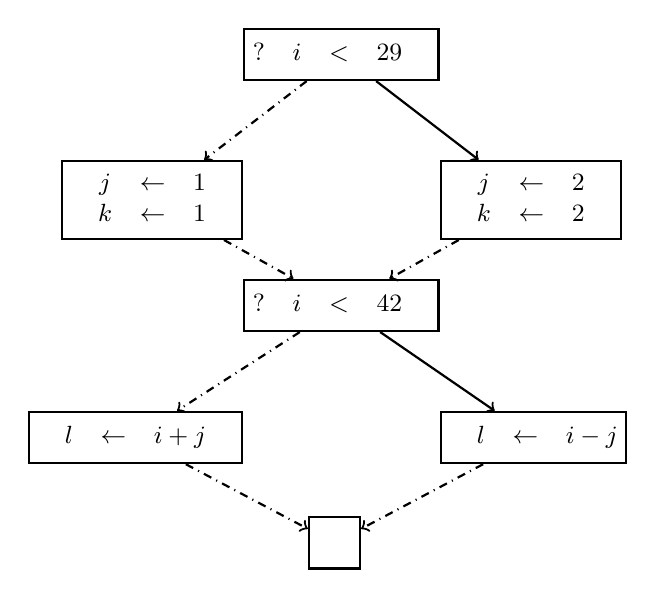
\begin{tikzpicture}
	\small
	  \node[block] (base) {$\begin{matrix*}
			? & i &<& 29 &\\
		  \end{matrix*}$
	   }; 
	  
	  \node[block, below left = 1cm and 0cm of base] (neg1) {
	  	$\begin{matrix*}
	  		&j &\gets& 1 &\\
	  		&k &\gets& 1 &
	  	\end{matrix*}$
	  }; 
	  
	  \node[block, below right = 1cm and 0cm of base] (pos1) {
		$\begin{matrix*}
			&j &\gets& 2& \\
			&k &\gets& 2&
		\end{matrix*}$
	  }; \&

	  \node[block, below = of {$(pos1)!0.5!(neg1)$}] (merge1) 		  			  {
	  $\begin{matrix*}
	  ? & i &<& 42 &\\
	  \end{matrix*}$
	  }; \&


	  \node[block, below left = 1cm and 0cm of merge1] (neg2) {
	  $\begin{matrix*}
	  &l &\gets& i + j &\\
	  \end{matrix*}$
	   
	  }; 
	  
	  \node[block, below right = 1cm and 0cm of merge1] (pos2) {
		$\begin{matrix*}
			&l &\gets& i - j \\
		\end{matrix*}$
		}; 
	  

	  \node[block, below = of {$(pos2)!0.5!(neg2)$}] (merge2) 		  			  {
	  $\begin{matrix*}

	  \end{matrix*}$
	  };

	% now link the nodes

	\draw [connector] (base) --  (pos1);
	\draw [dash dot, connector] (base) --  (neg1);
	\draw [dash dot, connector] (pos1) -- (merge1);
	\draw [dash dot, connector] (neg1) -- (merge1);
	\draw [connector] (merge1) -- (pos2);
	\draw [dash dot, connector] (merge1) -- (neg2);
	\draw [dash dot, connector] (pos2) -- (merge2);
	\draw [dash dot, connector] (neg2) -- (merge2);


  \end{tikzpicture}}
      \caption{Original form}
      \label{fig:ssa_before}
  \end{subfigure}
    \begin{subfigure}[t]{0.55\textwidth}
      \resizebox{\linewidth}{!}{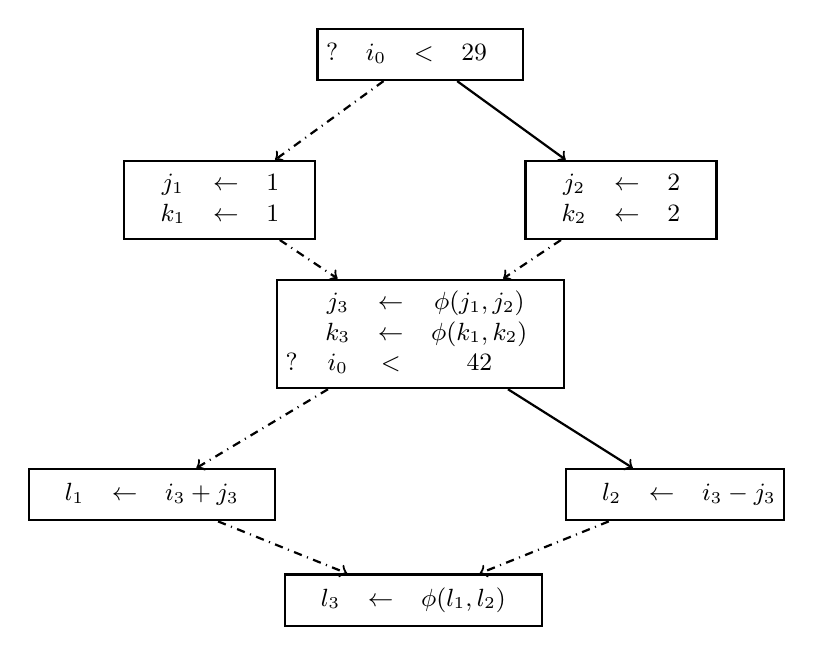
\begin{tikzpicture}
\small
  \node[block] (base) {$\begin{matrix*}
		? & i_0 &<& 29 &\\
	  \end{matrix*}$
   }; 
  
  \node[block, below left = 1cm and 0cm of base] (neg1) {
  	$\begin{matrix*}
  		&j_1 &\gets& 1 &\\
  		&k_1 &\gets& 1 &
  	\end{matrix*}$
  }; 
  
  \node[block, below right = 1cm and 0cm of base] (pos1) {
	$\begin{matrix*}
		&j_2 &\gets& 2& \\
		&k_2 &\gets& 2&
	\end{matrix*}$
  }; \&

  \node[block, below = of {$(pos1)!0.5!(neg1)$}] (merge1) 		  {
  	$\begin{matrix*}
  		&j_3 &\gets& \phi(j_1, j_2)& \\
  		&k_3 &\gets& \phi(k_1, k_2)& \\
  		? & i_0 &<& 42 &\\
  	\end{matrix*}$
  }; \&


  \node[block, below left = 1cm and 0cm of merge1] (neg2) {
  	$\begin{matrix*}
  		&l_1 &\gets& i_3 + j_3 &\\
  	\end{matrix*}$
   
  }; 
  
  \node[block, below right = 1cm and 0cm of merge1] (pos2) {
	$\begin{matrix*}
		&l_2 &\gets& i_3 - j_3 \\
	\end{matrix*}$
	}; 
  

  \node[block, below = of {$(pos2)!0.5!(neg2)$}] (merge2) 		  {
  	$\begin{matrix*}
		&l_3 &\gets& \phi(l_1, l_2)& \\
  	\end{matrix*}$
  };

% now link the nodes

\draw [connector] (base) --  (pos1);
\draw [dash dot, connector] (base) --  (neg1);
\draw [dash dot, connector] (pos1) -- (merge1);
\draw [dash dot, connector] (neg1) -- (merge1);
\draw [connector] (merge1) -- (pos2);
\draw [dash dot, connector] (merge1) -- (neg2);
\draw [dash dot, connector] (pos2) -- (merge2);
\draw [dash dot, connector] (neg2) -- (merge2);
\end{tikzpicture}}
        \caption{SSA form}
        \label{fig:ssa_after}
    \end{subfigure}
    \caption{SSA transformation}
    \label{fig:ssa}
\end{figure}

\subsubsection{Memory SSA}\label{memory-ssa}

As cited in the beginning of this section, the SSA form has a lot of
benefits, but is limited to scalar values and is not well suited for
compound structures such as arrays. One of the solutions to this problem
is Memory SSA as implemented by GCC {[}27{]}. This is a transformation
that runs on a sufficiently low-level representation of the source code,
where there's a notion of \texttt{LOAD} and \texttt{STORE} instructions.

Because the actual memory locations are not known during compilation
some abstractions are needed. GCC uses compiler symbols which they
called tags to represent regions of memory along with two virtual
operators \texttt{VDEF} and \texttt{VUSE}. For every \texttt{LOAD} a
\texttt{VUSE} of some tag(s) gets inserted, and likewise for
\texttt{STORE} and \texttt{VDEF}. There are three types of tags:

\begin{itemize}
\tightlist
\item
  \emph{Symbol Memory Tag} (SMT): These are the result of a
  flow-insensitive alias analysis and are almost purely type-based. For
  example, all dereferences of an \texttt{int*} receive the same tag to
  reflect the fact that they might point to the same memory location.
\item
  \emph{Name Memory Tag} (NMT): These are the result of a points-to
  analysis applied after the program is in a SSA form and inherits their
  flow-sensitive properties {[}27{]}. In other words, the GCC uses
  multiple different SSA forms.
\item
  \emph{Structure Field Tags} (SFT): These are symbolic names for the
  elements of structures and arrays.
\end{itemize}

Tags get used in a similar way as variables in the regular SSA
algorithm. Assigning to a tag is like assigning to all symbols that have
received that tag. In the original implementation, \emph{call
clobbering}, i.e.~a function call that alters the state of one of its
arguments such as in code sample \ref{smp:aliasing}, is handled the same
way as global variables {[}27{]}. All arguments that are known to get
clobbered sometimes are put into a single set. Calling functions that
would clobber one of them is assumed to clobber all of them. This
pessimistic approach has been replaced in recent implementations, where
all related code has been rewritten to use an \emph{aliasing-oracle}
{[}41{]}.

LLVM's usage of Memory SSA is not quite as documented. Their
documentation refers to GGC's paper {[}27, 47{]} and mentions that
\say{Like GCC’s, LLVM’s MemorySSA is intraprocedural.}. As mentioned in
the previous section, this isn't entirely true for GCC anymore. It
doesn't seem to be true for LLVM either. A recent publication describes
\emph{Static Value-flow} analysis which produces an interprocedural SSA
form {[}33{]}. It has been part of LLVM since 2016 and like GCC's
implementation it uses the results of an external points-to analysis.

\section{Symbolic Execution}\label{symbolic-execution}

Rather than using concrete values, symbolic execution uses symbolic
values. Those values represent possible values through a set of
constraints. This technique is commonly used to find interesting corner
cases for unit testing {[}5, 29, 31{]} and the original SSA paper used
similar principles to make their analysis more precise {[}2{]}.

At each branch point a \emph{path constraint} gets introduced, which is
a symbolic expression that must be true for the current branch to be
taken. If there are no values that satisfy all the constraints, the
branch gets flagged as dead code. In the case of a static analysis tool
this will most likely result in a warning, while a compiler would just
remove the dead branch. For example, consider code sample
\ref{smp:symb}. The condition \texttt{y\ \textgreater{}\ 0} becomes a
constraint during the execution of the positive branch, as well as
\texttt{x\ \textgreater{}\ -1}. The former constraint is pretty simple
to add, the latter requires some serious bookkeeping. Which implies a
close relation between symbolic execution and data-flow analysis.

\begin{code}
  \begin{tcblisting}{listing only, 
  arc=0pt,
  outer arc=0pt, 
  boxrule=0.2pt,
  minted language=python,
  minted style=autumn,
  minted options={xleftmargin=-6pt, linenos},
  colback=bg }
x = int(input())
y = x + 1

if y > 0:
    z = sqrt(y)
else:
    z = 0
\end{tcblisting}
\caption{Symbolic Execution} \label{smp:symb}
\end{code}

\vspace{-2pt}

Symbolic execution is a very powerful tool but comes with a few
limitations. One is the \emph{state explosion problem}. The number of
paths can increase very fast. The Java Pathfinder manages this problem
using state matching and backtracking {[}29{]}. State matching will
check if a similar state has already been processed. If it has, it will
backtrack to the next state that still has unexplored choices.

An advanced symbolic executor for Python is PyExZ3 {[}1, 3{]}, which is
built on top Microsoft Research's Z3 theorem prover. Z3 is a remarkably
good fit to reason about programming languages and even supports strings
and other sequences {[}26{]}. There are even extensions that add support
for regular expressions and other advanced constraints {[}39{]}. As
another team at Microsoft Research has pointed out however, sound
methods such as symbolic execution tend to run into problems when
applied to unsound languages {[}22{]}. Z3 heavily relies on type
information, which is not present in Python code. Lists and dictionaries
are still open challenges {[}3{]}, as Z3 requires an element type upon
declaring a sequence {[}26{]}.

\vspace{-1pt}

Symbolic executors typically focus on scalar values. Collections tend to
be a lot harder to analyze. Consider code sample \ref{smp:symb2} for
example, which defines a function \texttt{foo} that prints
\texttt{homogeneous} if and only if its argument is a collection and all
elements in that collection are of the same type. The positive branch
introduces a constraint on the length of \texttt{x}. Z3 can already
handle this quite well. The relation between uniqueness and the length
of a set is considerably harder though, and it's a very \emph{pythonic}
pattern.

\vspace{-1pt}

\begin{code}
  \begin{tcblisting}{listing only, 
  arc=0pt,
  outer arc=0pt, 
  boxrule=0.2pt,
  minted language=python,
  minted style=autumn,
  minted options={xleftmargin=-6pt, linenos},
  colback=bg }
def foo(x):
  if len(set(map(type, x))) == 1:
    print('homogeneous')
  else:
    print('heterogeneous')
\end{tcblisting}
\caption{Symbolic Execution Challenge} \label{smp:symb2}
\end{code}

\chapter{Fosite}\label{fosite}

There's a relatively unknown Frisian god of reconciliation, justice, and
mediation called Foseti. These are also some qualities that a good
static analyzer should aim to have as well to gain a user's trust
{[}4{]}. The analyzer developed as part of this thesis is called
Fosite,\footnote{\url{https://github.com/hdelva/fosite/tree/master} --
  accessed 31 May 2017} as foresight would be another good quality.

\section{Goals}\label{goals}

Unlike most existing tools, Fosite's focus is on analyzing small pieces
of code submitted by students that are new to programming, and this
comes with both advantages and disadvantages. The biggest advantage is
that we're free to explore slow but accurate methods. Not entirely free
however as feedback should still be fast. Imagine being a stressed out
student, working on your final exam and every submission takes a minute
to run because submissions come in faster than they get processed.

The most important requirement of all is that all warnings have to be as
helpful as possible. Providing the right details should make the
detection of errors more convincing and will be met with less resistance
from the user {[}4{]}. This is doubly important for new programmers;
simply pointing out bad style is not enough if the user does not know
how to fix it. Fosite therefore uses data-flow analysis to pinpoint the
source of problems and uses that information to inform the user.

\begin{code}
  \begin{tcblisting}{listing only, 
  arc=0pt,
  outer arc=0pt, 
  boxrule=0.2pt,
  minted language=python,
  minted style=autumn,
  minted options={xleftmargin=-6pt, linenos},
  colback=bg }
if x < y:
  z = x
else:
  z = y
\end{tcblisting}
\caption{Inefficient Implementations} \label{smp:shit}
\end{code}

We would like to be able to recognize suboptimal patterns as well, such
as in code sample \ref{smp:shit}. Replacing all occurrences of this
pattern with a call to \texttt{min} not only makes the code easier to
read, it's also significantly more performant in interpreted languages
such as Python. To be able to recommend sound code transformations, we
will rely on the research done in the area of compiler technology. The
analysis should also work as close as possible to the submitted code
though, and at the very least maintain a one-to-one relationship to it.
This is important because the end goal is automated refactoring, which
becomes hard when the input becomes mangled beyond recognition.

\section{Approach}\label{approach}

As pointed out in sections \ref{popular-languages} and \ref{compilers},
analysis of dynamic languages is often done using abstract interpreters,
and many modern compilers use an SSA form to perform sound
optimizations. The PyPy interpreter for Python constructs this form
using an abstract interpreter as well {[}48{]}, although their solution
is intraprocedural. Others have successfully used abstract interpreters
to perform a may-alias analysis on Python with the goal of optimization
{[}12{]}. Fosite is based on their conclusions and results, but it
ultimately has a different focus, i.e.~detailed static analysis and
automated refactoring.

The result of our analysis isn't exactly an SSA form for a few reasons.
The Memory SSA approach by the GCC and LLVM is a bad fit since it relies
on a low-level representation, which is a luxury we don't have as we
need to stay close to the original source code. Regular SSA is of course
an option since PyPy does it {[}48{]}, but can't handle collections
{[}27{]}.

Fosite emits more general \emph{use-def} information instead. A
\emph{use} refers to any data dependency, such as resolving a variable
name or retrieving an element from a collection. A \emph{def} is the
opposite such as assigning something to a variable name or inserting an
element into a collection. Within Fosite, a \emph{use} and a \emph{def}
are respectively called a dependency and a change. As with SSA,
incremental numbering can be applied to subsequent definitions. This can
be done in a similar fashion as applying the path convergence criterion
for the conversion to SSA form. The path-sensitivity of the analysis
already provides the necessary components to do so -- and control flow
is very well-structured in Python (and other dynamic languages). The
main difference with regular SSA is that this requires a separate data
structure. This allows a single expression or statement to cause
multiple changes. A conditional statement is exactly that -- a
statement, and it can be useful during refactoring to treat it as a
single atomic thing. Its dependencies and changes are the sum of its
branches'. In other words, the external data structure allows for a more
hierarchical analysis.

To achieve the same level of precision as Memory SSA, Fosite uses two
kinds of changes and dependencies. For starters, there's the usual
identifier dependency, which is used to model reachability of data.
Consider code sample \ref{smp:dep} in which \texttt{x} gets defined
twice. In between assignments, the first value of \texttt{x} gets used
in a call to \texttt{print}. The \texttt{print} must come before the
second assignment to \texttt{x}, as the intended data is no longer
reachable after the assignment. Another sort of dependency are object
dependencies, which are used to model state dependencies. The second
assignment to \texttt{x} assigns a list to it, which gets printed as
well. Before printing however an element gets appended to it. Appending
an element to a list doesn't change anything about the identifier and
thus can't be modeled in the same way. In other words, the final call to
\texttt{print} has a dependency to both the \texttt{x} identifier and to
whichever object \texttt{x} points to at the same time -- and both
dependencies serve their own purpose.

\begin{code}
  \begin{tcblisting}{listing only, 
  arc=0pt,
  outer arc=0pt, 
  boxrule=0.2pt,
  minted language=python,
  minted style=autumn,
  minted options={xleftmargin=-6pt, linenos},
  colback=bg }
x = int(input())
y = int(input())
print(x - y)

x = []
x.append(1)
print(x)
\end{tcblisting}
\caption{Dependency Example} \label{smp:dep}
\end{code}

There are hidden dependencies in this program as well. The first two
lines of code will read two lines from \texttt{stdin} and parse them to
integers. The order in which this happens is important, since the two
values get subtracted from each other. This can be modeled by adding
implicit state. The call to \texttt{input} both depends on the implicit
state and changes it, which will ensure that the relative order between
the two calls remains the same. Other IO functionality such as the
\texttt{print} call will do the same. Implicit state can easily be
modeled by designating a specific and hardcoded object to be the
internal state.

\section{Languages}\label{languages}

Since programming languages tend to share a lot of features, it's not
unthinkable to have an abstract interpreter that can process multiple
languages. The first thing this would need is a common input format,
which in Fosite's case is its \emph{General Abstract Syntax Tree}
(GAST). It has to be able to capture all \emph{syntactic} features of
the languages it supports -- the semantics aren't relevant for an AST.
Adding support for an additional language will require some new nodes or
some extra information in existing nodes. Since only things will have to
get added interpreting the existing languages can just ignore the
additional node types. Another thing that's special about the GAST is
that every node has its unique identifier, and the identifiers are
totally ordered. If one node's identifier is less than another's, that
must mean it came before that other node in the original source file.
This is important to accurately report code points, but also because
some optimizations rely on it.

The interpreter has to be able to add semantics to the common AST
structure. A different \texttt{Executor} instance may be assigned for
every supported node for every supported language. Languages that share
the same features can reuse existing \texttt{Executor} implementations.
Common and fundamental features such as function scoping are even
available inside the interpreter's implementation itself.

As the test data itself is in Python, the Python programming language
was the main focus during implementation.

\section{Analysis}\label{analysis}

While linters recognize error prone patterns, an interpreter can
recognize error prone patterns and logic, as well as some outright
errors. An additional benefit of an interpreter-based approach is that
it approaches feedback the same way a person would: starting at the
beginning, step by step. There are some interesting things that an
interpreter can do that linters (or at least PyLint) can't.

\begin{code}
  \begin{tcblisting}{listing only, 
  arc=0pt,
  outer arc=0pt, 
  boxrule=0.2pt,
  minted language=python,
  minted style=autumn,
  minted options={xleftmargin=-6pt, linenos},
  colback=bg }
def foo():
    for ...:
        for ...:
            if ...:
                return ...
            elif ...:
                return ...
\end{tcblisting}
\caption{Function Returns} \label{smp:return}
\end{code}

Code sample \ref{smp:return} contains an error prone pattern of
Python-like code. A student had written something like this which
resulted in one out of 200 unit tests failing. Written like this, it's
possible that none of the intended \texttt{return} statements are
executed. If this happens, the return value is going to be
\texttt{None}, which makes the unit test fail in an unexpected way --
nowhere did they specify a \texttt{None} value should be returned.
Fosite gives an accurate description of the cause -- the function did
not return under these conditions -- instead of just the result.

\begin{code}
  \begin{tcblisting}{listing only, 
  arc=0pt,
  outer arc=0pt, 
  boxrule=0.2pt,
  minted language=python,
  minted style=autumn,
  minted options={xleftmargin=-6pt, linenos},
  colback=bg }
x = []
...
while tuple([0] * i) not in x:
    ...
    x += tuple([0] * i)
\end{tcblisting}
\caption{Heterogeneous Collections} \label{smp:nohomo}
\end{code}

The test data contains an exercise that required that a sequence of
tuples should be generated, stopping whenever a tuple of zeroes has been
added. Code sample \ref{smp:nohomo} is based on one of the submissions.
Up until the addition of the tuple of zeroes, the type of \texttt{x} had
been \texttt{List{[}Tuple{[}int{]}{]}} (in the notation used by Python
3.5 type hints). Instead of appending the tuple however, \texttt{+=}
will concatenate the tuple's elements to \texttt{x} -- in the same way
calling \texttt{extend} on \texttt{x} would. This changes the type to
\texttt{List{[}Union{[}int,\ Tuple{[}int{]}{]}{]}}. This transition to a
heterogeneous collection is valid Python code but ultimately very error
prone. In fact, this causes an infinite loop in this case, as the
expected element never gets added.

\begin{code}
  \begin{tcblisting}{listing only, 
  arc=0pt,
  outer arc=0pt, 
  boxrule=0.2pt,
  minted language=python,
  minted style=autumn,
  minted options={xleftmargin=-6pt, linenos},
  colback=bg }
def change(x, d = None):
  list1 = ''
  list2 = []
  for i in range(0, len(x)):
    while x[i] != ' ':
      list2 += x[i]
    list1 += translate(list2[0], d)
    list2 = []
  return list1
\end{tcblisting}
\caption{Endless Loop} \label{smp:nostop}
\end{code}

Although deciding whether or not any given program will stop is
impossible, it is possible in some cases. Those cases also happen to be
quite common. Code sample \ref{smp:nostop} is an excerpt from a
submission. The student intended to tokenize the string \texttt{x},
building the token in \texttt{list2}. Every token should then get
translated and the translated token gets stored in \texttt{list1}. There
are a number of mistakes, but the most important one is the endless
\texttt{while} loop. The student wanted index \texttt{i} to be a
starting position of the token, with the \texttt{while} loop building
the token from that point. That's of course not what the code does. The
same character will get added over and over since none of the values in
the loop condition ever change. Data-flow analysis remembers when and
where variables get their values, so it can be used to recognize that
the variables are still the same.

The secondary goal of the interpreter is to open the door to code
refactoring, through the means of a data-flow analysis. Every evaluated
node during interpretation emits a list of changes and dependencies as
discussed in section \ref{approach}.

\chapter{Implementation}\label{implementation}

Fosite is an abstract interpreter. It uses abstract pointers, which can
be used to fetch abstract objects from an abstract memory. The objects
themselves have no value, but they do have a notion of types,
attributes, and elements. There is a notion of namespaces where names
get mapped to objects, and a notion of heterogeneous collections. In
essence, the interpreter tries to get as close as it can to an actual
interpreter, without having actual values. This is not as obvious as it
sounds. For example, it's tempting to cut corners when implementing the
\emph{Method Resolution Order} (MRO), variable capturing in closure
definitions, or the explicit \texttt{self} argument in Python. Simple
approximations of these behaviors would suffice for well written code --
but targeting such code makes no sense for a static analyzer. We have to
be able to analyze \emph{really} bad code as well.

\begin{code}
  \begin{tcblisting}{listing only, 
  arc=0pt,
  outer arc=0pt, 
  boxrule=0.2pt,
  minted language=python,
  minted style=autumn,
  minted options={xleftmargin=-6pt, linenos},
  colback=bg }
x = 0
y = 0
z = 0

if ...:
    x = 9
    if ...:
        y = 5
        if ...:
            z = 1

a = complex_computation(x)
b = complex_computation(y)
c = complex_computation(z)
\end{tcblisting}
\caption{State Explosion} \label{smp:branch}
\end{code}

As an abstract interpreter uses abstract values, it can't decide which
branch to take at every branch point, so it will explore every possible
branch. This can quickly lead to a state explosion problem as the number
of branches can increase exponentially. Consider the Python-like code in
code sample \ref{smp:branch}. There are branching points on lines 5, 7
and 9, so that the function calls on lines 12, 13, and 14 can each be
executed once for each of the four possible execution paths for a total
of 12 calls to \texttt{complex\_computation}. Each argument \texttt{x},
\texttt{y} or \texttt{z} only has two possible values though, so we
should be able to do better. The Fosite interpreter will create new
execution paths at every branch point, but those paths will also be
merged after evaluating the branch point. This means that there will
only be a single active execution path left upon executing the calls on
lines 12-15. Merging execution paths preserves all the relevant
information of each branch, as discussed in section \ref{namespace}. The
result still has exponential complexity, but no longer in the number of
branch points but in the number of possible values

\section{Objects}\label{objects}

As alluded to at the beginning of section \ref{implementation}, the
Fosite interpreter keeps track of attributes and elements. Attributes
can reuse the namespace logic as described in sections \ref{namespace}
and \ref{name-resolution}. Elements are a lot harder to model and are
covered in section \ref{collections}.

Everything is an object in Python, even classes become class objects
upon definition. An object of a class has a reference to its class
object. Among other things, this reference gets used during name
resolution. Every class can also extend multiple other classes, called
base classes, in a similar way. This can easily be modeled in an
abstract interpreter using a list of pointers.

The type of an object is harder to model however. In many
object-oriented languages, an object's class is its type. Python's
situation is a bit more complex since it has multiple inheritance, and
classes are objects as well.

\begin{code}
  \begin{tcblisting}{listing only, 
  arc=0pt,
  outer arc=0pt, 
  boxrule=0.2pt,
  minted language=pycon,
  minted style=autumn,
  minted options={xleftmargin=-6pt, linenos},
  colback=bg }
>>> x = 42
>>> t1 = type(x)
>>> t1
<class 'int'>
>>> t2 = type(t1)
>>> t2
<class 'type'>
>>> t3 = type(t2)
>>> t3
<class 'type'>
\end{tcblisting}
\caption{Types in Python} \label{smp:types}
\end{code}

Code sample \ref{smp:types} illustrates why this is odd. The
\texttt{type} function returns a class object, so that \texttt{type(42)}
returns the class object of name \texttt{int}. Using the same function
to get the class object's type returns a class object of name
\texttt{type}. Requesting that object's type reveals something strange
-- \texttt{type} is its own type. This seemingly cyclic dependency gets
implemented in CPython using a type flag, if that flag is set it will
return the type class object when needed. In other words, the
\texttt{type} object doesn't have a reference to itself, it will get a
reference to itself at runtime when needed.

The type of a value is the same as its class object. A class's basetypes
have nothing to do with its type -- a class object's type is always
\texttt{type}. These semantics are quite straightforward to model in an
abstract interpreter: the list of base class references are still there,
but there's also a type flag. When that flag is set, the \texttt{type}
function shouldn't use the base classes but fetch the pointer to the
\texttt{type} class object.

\section{Paths and Mappings}\label{paths-and-mappings}

In order to accurately report the cause of errors and warnings, we need
to know the source of every value. A path corresponds to a sequence of
code points so that the user gets an idea of the execution path that
leads to a problem. A path is an ordered sequence of path nodes.
Examples of path nodes include which branch of a conditional was
followed, assignments, and function calls. The path nodes should submit
a logical ordering, so that users can easily interpret results. For
example, this is what a path may look like to the users:

\begin{tcblisting}{listing only, 
  arc=0pt,
  outer arc=0pt, 
  boxrule=0.2pt,
  minted language=fosite,
  minted style=manni,
  minted options={},
  colback=bg }
Call to numismatist at row 113, column 1
Element of the collection at row 97, column 9
Call to repeater at row 98, column 16
Assignment to lijst at row 113, column 1
Assignment to i at row 97, column 9
Assignment to getal at row 98, column 16
\end{tcblisting}

As mentioned in section \ref{languages}, AST nodes have totally ordered
unique identifiers. A first attempt at defining the path node would be
to just reuse the AST identifiers. This works fine until function calls
come into the picture. A function call will come after the function
definition, and its identifier will be larger than any of the function
definition's nodes. This would place the execution of the function body
before the function call itself. On top of that, this approach does not
support executing the same node more than once. A better solution is to
define a path node to be an ordered collection of AST nodes -- the nodes
that are currently being executed. Some nodes need extra information. A
conditional branch node for example needs to indicate which branch was
actually taken. Each branch is incrementally numbered, and contains the
total number of branches for practical reasons (see sections
\ref{namespace} and \ref{function-calls}). The actual branch numbers are
of no concern. Their main purpose is telling possible branches apart.

Definition \ref{def:path_node} describes the structure of a path node,
and definition \ref{def:path_order} defines how path nodes are ordered.
Note that \(\prec\) is the symbol meaning ``precedes'', and
\(\prec_{lex}\) means it precedes according to the lexicographic
ordering. Definition \ref{def:contain} defines a property which will get
used in section \ref{conditionals} where it will be used to exclude
results because they contain paths that would contradict the current
execution path.

If we have to merge two paths at any point during execution, we'll need
to make sure the paths are mergeable at all. This is important when
evaluating binary operations, or during name resolution of an attribute.
Definition \ref{def:complement} contains the definition of any given
node's complementary nodes. Definition \ref{def:mergeable} says that two
paths are mergeable if neither path contains nodes that complement any
other the other's path nodes. A path's complementary paths can be
constructed using the complements of its nodes, this process is
described in algorithm \ref{alg:complement}. Complementary paths will
prove useful in section \ref{loops}.

\begin{definition} \label{def:path_node}
A path node is of the form $((n_1, n_2, ... , n_i), b, t)$, where the elements $n_i$ are an ordered sequence of AST node identifiers, $b$ is the number of the branch that was taken, and $t$ is the total of branches that were possible at that node.
\end{definition}

\begin{definition} \label{def:path_order}
Let $p$ and $q$ be two path nodes with forms respectively $(n_p, b_p, t_p)$ and $(n_q, b_q, b_t)$, $p \prec q \iff n_p \prec_{lex} n_q \vee (n_p = n_q \wedge b_p \prec b_q )$. 
\end{definition}

\begin{definition} \label{def:contain}
A path $A$ is \textit{contained} in another path $B$ if every node of path $A$ occurs in path $B$ as well.
\end{definition}

\begin{definition} \label{def:complement}
The complementary nodes of a single path node $(n_p, b_p, t_p)$ are defined as $\{\, (n_p, i, t_p) \mid 0 \leq i < t \wedge i \neq b_p \,\}$. If $t_p = 1$, an assignment node for example, there are no complementary nodes.
\end{definition}

\begin{definition} \label{def:mergeable}
A path $A$ is \textit{mergeable} with another path $B$ if a $A$ does not contain a complement of one of $B$'s nodes. \end{definition}

\begin{algorithm}
    \caption{Complementary Paths}\label{alg:complement}
    \begin{algorithmic}[1]
        \Function{complement} {path}
          \State $\texttt{result} \gets [\,]$
          \State $\texttt{current} \gets [\,]$
          \ForAll{nodes in path}
            \If{ $\texttt{node.is\_branch()}$ }
              \ForAll{complements of node}
                \State $\texttt{temp} = \texttt{current.clone()}$
                \State $\texttt{temp.add\_node(complement)}$
                \State $\texttt{result} \gets \texttt{result} \cup \texttt{temp}$
              \EndFor
            \EndIf
            \State $\texttt{current.add\_node(complement)}$
          \EndFor
          \Return result
        \EndFunction
    \end{algorithmic}
\end{algorithm}

A mapping is simply a pair of the form \texttt{(Path,\ Pointer)}.
Because they usually appear in multiples, they can be implemented as a
list of \texttt{(Path,\ Pointer)} values instead. In this case, every
path in a mapping must be distinct. There are no paths that are
contained by another path in the same mapping.

\section{Boolean Expressions}\label{boolean-expressions}

A boolean expression can be arbitrarily hard to evaluate. When used in a
conditional statement, we can't always decide whether or not a given
branch gets taken. The best we can do in these cases is concluding that
the branch \emph{might} get taken. Evaluating any boolean expression can
thus result in \texttt{True} or \texttt{False}, as well as
\texttt{Maybe}.

\begin{code}
  \begin{tcblisting}{listing only, 
  arc=0pt,
  outer arc=0pt, 
  boxrule=0.2pt,
  minted language=python,
  minted style=autumn,
  minted options={xleftmargin=-6pt, linenos},
  colback=bg}

if current is not None:
  print('given {}-{}'.format(current.year, current.month))
else:
  current = datetime.now()

\end{tcblisting}
\caption{Conditions} \label{smp:conds}
\end{code}

Code sample \ref{smp:conds} shows that in some cases, we really need an
accurate answer. This is a pattern that occurs when dealing with
optional arguments or when writing library functions. The negative
branch should only get executed when \texttt{current} was not
\texttt{None}, so that an actual argument doesn't get overwritten. On
the other hand, it \emph{must} be executed if \texttt{current} was
\texttt{None}, so that further evaluation doesn't result in a false type
error.

The \texttt{is} operator compares the addresses of two objects and
returns \texttt{True} if and only if they're equal. We can mimic this
behavior -- and answer with certainty and under which conditions the two
operands' point to the same location. The resulting mapping will use the
merged paths of the operands to point to the \texttt{True} object. The
\texttt{==} operator should be similar. Technically it depends on the
implementation of the \texttt{\_\_eq\_\_} method, but let's assume that
it has a decent implementation. In that case it should at least return
\texttt{True} if both operands point to the same object -- as with
\texttt{is}. A similar reasoning can be applied to the \texttt{!=},
\texttt{\textless{}=}, and \texttt{\textgreater{}=} operators.

We can also handle the \texttt{and}, \texttt{or}, and \texttt{not}
operators in a similar way. If both operands already point to
\texttt{True}, we can merge the paths and return a mapping that points
to \texttt{True} as well. The other two operators are analogous.

We combine the paths of both operands to get a new mapping. This means
that we must only consider path pairs that are mergeable. Failing to
meet this requirement will lead to false positives very quickly.

\section{Conditionals}\label{conditionals}

Evaluating the test of a conditional branch can give us useful
information for the evaluation the individual branches. If that
information includes for example that we are sure that \texttt{x} is not
\texttt{None}, we should disregard any mapping that says otherwise. Even
better, we can exclude any mapping that would occur under the same
contradictory conditions -- even if those mappings don't have an
explicit connection to \texttt{x}.

\begin{code}
  \begin{tcblisting}{listing only, 
  arc=0pt,
  outer arc=0pt, 
  boxrule=0.2pt,
  minted language=python,
  minted style=autumn,
  minted options={xleftmargin=-6pt, linenos},
  colback=bg}
if cond1: # Condition 1
  y = None
  z = None
  
if y is not None: # Condition 2
  print(z.attribute)

\end{tcblisting}
\caption{Conditions} \label{smp:exclude}
\end{code}

In code sample \ref{smp:exclude}, there's an implicit relation between
condition 1 and condition 2. Going back to section
\ref{boolean-expressions}, the result of the test of condition 2 will
contain a mapping \((p, x)\), where \(p\) contains a node indicating
that the positive branch of condition 1 was taken, and where \(x\) is a
pointer value to \texttt{False}. This means that any mapping containing
\(p\) during the execution of the positive branch of condition 2 cannot
occur during actual execution. We will call this concept
\textit{path exclusion}, and paths such as \(p\) are called
\emph{restricted paths}. Observation \ref{obs:exclude} summarizes this
more formally.

\begin{observation}
\label{obs:exclude}
Assume that resolving an identifier $x$ results in a set of mappings $M$. Every mapping $m \in M$ is of the form $(p, a)$, where $a$ is a pointer value, and $p$ is the execution path that mapped $x$ to $a$. 

Let $R$ be the set of restricted paths. Given a mapping $(p_m, a) \in M$, if there exists a path $p_r$ in $R$ for which holds that $p_m$ contains $p_r$ (by definition \ref{def:contain}), we can exclude the mapping from the current evaluation. 
\end{observation}

\section{Loops}\label{loops}

Without being able to accurately evaluate loop conditions or generators
it's impossible to know how many times a loop body gets executed. There
are a few different approaches to this problem. The most accurate one is
to iterate until we can conclude doing further iterations won't benefit
the analysis anymore, we say that a \emph{fixed-point} state has been
reached in this case. Every iteration will likely change something
though, so that recognizing a fixed-point state isn't as easy as waiting
for an iteration that changes nothing.

An easier approach that still has sufficient accuracy is to evaluate
every loop body exactly twice. Theoretically it's possible to not even
do a single iteration -- this leads to false positives however as most
exercises can guarantee that some loops will always have to do
something. There are two reasons why two iterations is significantly
more accurate than a single one. For starters, the first iteration can
redefine values that are only used within the loop body. If this
redefinition is wrong, this can only be recognized by evaluating it a
second time. The second reason is to differentiate between the
\texttt{break} and \texttt{continue} statements. As section
\ref{namespace} will discuss, these two statements will hide changes
until some later point during execution. For the \texttt{break}
statement that point is the end of the loop, for the \texttt{continue}
statement however this point is the beginning of the next iteration.

The analysis of loops goes hand in hand with \emph{watches}, which are
used to compare the execution state before and after executing the loop.
They start in a setup phase, during which they will learn which
components to watch. A new watch gets made at the beginning of
evaluating the loop test or loop generator, and it will store all data
dependencies (corresponding to those of the data-flow analysis) for that
expression. It will contain the returned mappings for the identifiers,
along with a list of used objects. The watch leaves the setup phase
before evaluating the loop body, and it will now store all data changes
for the identifiers and objects that are being watched.

The information in a watch can be used to see whether or not iterating
affects the loop test or the loop generator. Knowing under which
conditions iteration changed something is easy. The watch already
contains that information. Finding the paths that don't change anything
isn't as easy because the watches only contain changes -- the opposite
of what we want. The invariants can be found by taking all the
complementary paths of all the changes, and retaining only those that
are mergeable with all changes. Section \ref{warnings} will discuss how
this information can be used as an indicator of error prone code.

\section{Namespace}\label{namespace}

Namespaces are the most essential component of the interpreter. We want
to give the most descriptive and helpful messages we can, by describing
the conditions in which something occurs. Paths are a first step towards
describing these conditions, but namespaces are where they're stored.
There are a few layers of abstraction required to make this possible,
and they will be introduced incrementally.

\subsubsection{OptionalMapping}\label{optionalmapping}

Mappings have already been introduced, but they contain a pointer value
which is not enough to indicate an uninitialized variable. A different
structure is used to this end, where the pointer value is optional. An
\texttt{OptionalMapping} with a missing pointer value indicates an
uninitialized variable and also describes why the variable is
uninitialized.

\subsubsection{Branch}\label{branch}

The \texttt{Branch} struct is the first layer of a namespace and it's
where names are added, its internal structure is of the form
\texttt{HashMap\textless{}String,\ OptionalMapping\textgreater{}}. Every
branching point during execution can induce several new branches in a
namespace that are separated during execution, so that the negative and
the positive branch of a conditional statement do not influence each
other for example. A \texttt{Branch} struct only contains the changes
that happened in its own branch. The changes that happened before
branching are stored in different \texttt{Branch} structs, which leads
to a sparse data structure.

\subsubsection{StatisChamber}\label{statischamber}

If we encounter a \texttt{break} statement while evaluating a loop body,
the evaluation of the current execution path terminates. The changes
made until that point have to be saved, as they will become relevant
after the loop has been evaluated. Function calls require the same to
handle different return points. A \texttt{StatisChamber} contains a
\texttt{HashMap\textless{}Path,\ Branch\textgreater{}}. The path key is
used because the control flow can be broken at multiple points.

\subsubsection{SubFrame}\label{subframe}

For every branch point, we use a \texttt{Branch} and three
\texttt{StatisChamber}s -- two for loops, one for function calls. Loops
require two statis chambers to keep the ones caused by a
\texttt{continue} separate from those caused by a \texttt{break}. These
four components get stored in a \texttt{SubFrame} struct.

\subsubsection{Frame}\label{frame}

This is the first namespace component that contains some actual logic.
Every branch point leads to the creation of a new \texttt{Frame}. This
structure contains a \emph{cause}, the path node where the branching
happened. It also contains a subframe for each possible branch at the
cause node. There is only one subframe active at any point during
execution and its index is stored. Algorithm \ref{alg:setframe}
describes how a mapping gets inserted into a frame. The \texttt{insert}
method of a \texttt{StatisChamber} will simply insert into each of its
branches.

\begin{algorithm}
    \caption{Set Mapping}\label{alg:setframe}
    \begin{algorithmic}[1]
        \Function{set\_mapping} {name, mapping}
          \If{ $\texttt{self.contains(name)}$ }
            \State $\texttt{old\_mapping} \gets \texttt{self.resolve(name)}$
          \Else
            \State $\texttt{old\_mapping} \gets \texttt{OptionalMapping}::new(\texttt{Path}::empty(), None)$
          \EndIf
        
          \State $\texttt{self.current\_branch.loop\_statis.insert(name, old\_mapping)}$
          \State $\texttt{self.current\_branch.function\_statis.insert(name, old\_mapping)}$
          \State $\texttt{self.current\_branch.branch.insert(name, mapping)}$
        \EndFunction
    \end{algorithmic}
\end{algorithm}

\begin{code}
  \begin{tcblisting}{listing only, 
  arc=0pt,
  outer arc=0pt, 
  boxrule=0.2pt,
  minted language=python,
  minted style=autumn,
  minted options={xleftmargin=-6pt, linenos},
  colback=bg}
# frame 1
x = 'x'
y = 'y'

while True:
    if 'cond': 
        # frame 2, subframe 2.1
        if 'cond2': 
            # frame 3, subframe 3.1
            x = 9
            continue
    else:
        # frame 2,subframe 2
        if 'cond4': 
            # frame 4, subframe 4.1
            y = 7
            break

    z = x + y

z + 'z'
\end{tcblisting}
\caption{Broken Control Flow} \label{smp:statis}
\end{code}

Code sample \ref{smp:statis} illustrates how the statis chambers are
used. When executing the \texttt{continue} statement on line 11, the
active branch will only contain a mapping for \texttt{x} in which it
points to an \texttt{int} object. This will stop the current execution
path, and conclude the execution of the conditional on line 6 as it does
not have a negative branch. Rather than merging the contents of subframe
\texttt{3.1} into subframe \texttt{2.1}, it will put the contents into
the loop static branch of subframe \texttt{3.1}. The key used to store
into the statis chamber is a path containing only a single node: the
node corresponding to the positive branch of line 8.

The first time the addition on line 19 gets executed is actually safe --
\texttt{x} and \texttt{y} will always have type \texttt{str} at this
point, and \texttt{z} will also receive a mapping to an object of type
\texttt{str}. Every loop gets evaluated twice as discussed in section
\ref{loops}, and a mapping in which \texttt{x} points to an \texttt{int}
since line 10 in the previous iteration is now part of the active
branch.

Line 21 isn't safe either. There are at least two execution paths that
left \texttt{z} uninitialized: if either the condition on line 8 or the
one on line 14 was true. Before the addition on line 19 was executed,
the previous value was stored into the statis chambers that existed at
the time. All but one statis chamber will now contain an empty mapping
for \texttt{z}, indicating an uninitialized value. These mappings enter
the active branch at the end of evaluating the loop, to give us the
wanted analysis result.

\subsubsection{Namespace}\label{namespace-1}

The actual namespace is simply a list of frames, one for each branch
point that is being executed. Looking up an identifier is simple: look
for the most recent frame that contains a mapping for that name. Name
resolution is simple because the other operations do all the heavy
lifting. There are three other operations:

\begin{itemize}
\tightlist
\item
  \textit{Grow}: Uses a path to create new frames until there is a frame
  for each node in the path.
\item
  \textit{Insert}: Grows the namespace when needed and then inserts a
  mapping into the last frame.
\item
  \textit{Merge}: Merges the last frame into the previous frame.
\end{itemize}

For the sake of data sparsity, growing is done upon insertion -- and not
upon the actual branching. Bearing in mind that every object has a
namespace as well, we don't want to grow each of their namespaces every
time -- its namespaces probably won't even change as most objects are
immutable literals.

\subsubsection{Grow}\label{grow}

If the current namespace has \(n\) frames, and the given path has \(m\)
nodes, we must add \(m-n\) frames -- corresponding to the last \(m-n\)
path nodes. The correctness of this approach relies on a bit of
inductive reasoning.

The active execution path will always be at least as long as the number
of frames in any namespace. All the namespaces that have been changed
have the same number of frames. If a change has been made in the current
branch, growing has added frames until there are as many frames as there
are nodes in the execution path. If a change was made in some branch
that is already been executed, and is thus no longer part of the
execution path, merge operations will have reduced the number of frames
until the length is equal to the length of execution path. The
namespaces that have not been changed have strictly less frames,
corresponding to the length of the execution path of their last change.

The causal nodes of the frames of any namespace form a prefix of the
active execution path. This is a trait of the language. Since Python (or
any other language we would target) does not have a \texttt{goto}
statement, there is a fixed structure to the branching points.

\subsubsection{Merge}\label{merge}

The merge operation combines the results of the last frame, removes it,
and puts the merged result into the frame that is now last. An argument
determines the destination of every subframe's content -- either into
the regular branch or into a statis chamber. The current method is
specific to function scoping, but block scoping can be added in a
similar way.

\begin{code}
  \begin{tcblisting}{listing only, 
  arc=0pt,
  outer arc=0pt, 
  boxrule=0.2pt,
  minted language=python,
  minted style=autumn,
  minted options={xleftmargin=-6pt, linenos},
  colback=bg }
x = 42
y = 'string'

if cond:
  x = '42'

x + y 
\end{tcblisting}
\caption{Merging}\label{smp:merge}
\end{code}

The name resolution stops at the most recent frame that contains that
name. Code sample \ref{smp:merge} illustrates that this isn't just an
easy solution -- it can also be a useful one. If the negative branch of
the condition at line 4 is taken, execution will fail at line 7.
Variable \texttt{x} still has the value it received at line 1, but only
reporting this paints an incomplete picture. It only has that value if
the negative branch was taken. So if we want to accurately describe why
it has that value, that information should be there as well.

\begin{algorithm}
    \caption{Merge}\label{alg:merge}
    \begin{algorithmic}[1]
        \Function{merge} {}
          \State $\texttt{names} \gets [\,]$

          \ForAll{ subframes \textbf{in} frames.last()}
            \State $\texttt{names} \gets \texttt{names} \cup \texttt{subframe.names}$
          \EndFor

          \State $\texttt{branch\_content} \gets \texttt{Branch}::new()$

          \State $\texttt{loop\_statis} \gets \texttt{StatisChamber}::new()$

          \State $\texttt{function\_statis} \gets \texttt{StatisChamber}::new()$

          \State $\texttt{cause} \gets \texttt{frames.last().cause}$

          \ForAll{ (i, subframes) \textbf{in} frames.pop().enumerate()}
            \State $\texttt{new\_node} \gets \texttt{PathNode}::new(\texttt{cause, i})$
            \State $\texttt{subframe.augment\_statis\_chambers(new\_node)}$
            \State $\texttt{loop\_statis.insert\_all(subframe.loop\_statis)}$
            \State $\texttt{function\_statis.insert\_all(subframe.function\_statis)}$
            \ForAll{name}
              \State $\texttt{mapping} \gets \texttt{subframe.resolve(name)}$
              \State $\texttt{mapping.augment(new\_node)}$

              \If { \texttt{break\_loop(subframe)}}
                  \State $\texttt{loop\_statis.add(mapping)}$
              \Else 
                \If { \texttt{return\_function(subframe)}}
                    \State $\texttt{function\_statis.add(mapping)}$
                \Else 
                    \State $\texttt{branch\_content.add(mapping)}$
                \EndIf
              \EndIf
            \EndFor
          \EndFor

          \State $\texttt{frames.last().insert\_all(branch\_content)}$
          \State $\texttt{frames.last().insert\_all\_loop\_statis(loop\_statis)}$
          \State $\texttt{frames.last().insert\_all\_function\_statis(function\_statis)}$
        \EndFunction
    \end{algorithmic}
\end{algorithm}

Merging begins with collecting the names of all identifiers that have
changed in each branch of the frame. A variant of the cause node gets
created for every subframe, using the index of the subframe. These
augmented nodes are then used to \emph{augment} the paths in the statis
chambers, which then get moved to the frame that is now last. The statis
chambers are all of the form
\texttt{HashMap\textless{}Path,\ Branch\textgreater{}}, where the
\texttt{Path} was supposed to keep the different sources of broken
control flow apart. The \texttt{augment} method will add a new node to
every key path -- future additional key paths won't contain this node,
which is how different points of broken control flow are being kept
separate.

Code sample \ref{smp:merge} showed us some behavior we want during name
resolution. We can achieve this by incorporating name resolution in the
merge operation. Every identifier that has been changed in any branch
will get resolved in every branch, the result gets augmented gets
augmented with a variant of the cause node, and is then stored in the
frame that is now last. This will ensure that all the relevant mappings
for any given identifier can always be found in a single frame. More
importantly, the \texttt{augment} method will update path mappings to
reflect when an identifier didn't change in some particular branch.

Function calls and loops can also create a new frame in namespaces.
While merging after a conditional branch can place things inside a
statis chamber, merging after a loop or a function call will place the
contents of a statis chamber into the active branch. The key paths are
merged into the mappings of their corresponding branches first because
previous merge operations have not updated those mappings yet.

\section{Name Resolution}\label{name-resolution}

Namespaces by themselves aren't enough to implement all the name
resolution behavior; name resolution uses several namespaces. It's
possible that a variable is sometimes uninitialized in a namespace, in
which case resolution can continue using another namespace. The
unresolved paths are carried over to the resolution in the next
namespace. All returned mappings have their paths merged with the
unresolved paths to reflect the fact that name resolution continued in
the next namespace. Algorithm \ref{alg:chain} illustrates the general
method of name resolution, the \texttt{next\_namespace} function depends
on the kind of name being resolved. An error is emitted if
\texttt{unresolved} is not empty and there are no more namespaces to
try.

\begin{algorithm}
    \caption{Resolve}\label{alg:chain}
    \begin{algorithmic}[1]
        \Function{resolve} {name}
          \State $\texttt{result} \gets \texttt{Mapping}::new()$

          \State $\texttt{unresolved} \gets [\, \texttt{Path}::empty()\,]$

          \While{ \texttt{unresolved.len() > 0} }
              \State $\texttt{new\_unresolved} \gets [\,]$

              \State $\texttt{namespace} \gets \texttt{next\_namespace()}$
              \State $\texttt{mapping} \gets \texttt{namespace.resolve(name)}$

              \ForAll{$(p, x)$ \textbf{in} mapping}
                \ForAll{ \texttt{unresolved\_path} \textbf{in} \texttt{unresolved}}
                    \State $\texttt{new\_path} \gets \texttt{p.merge(unresolved\_path)}$

                    \If {\texttt{x.is\_none()}}
                      \State $\texttt{new\_unresolved} \gets \texttt{new\_unresolved} \cup \texttt{new\_path}$
                    \Else 
                      \State $\texttt{result.add(new\_path, x)}$
                    \EndIf
                \EndFor
              \EndFor

              \State $\texttt{unresolved} \gets \texttt{new\_unresolved}$

          \EndWhile

          \State \Return \texttt{result}
        \EndFunction
    \end{algorithmic}
\end{algorithm}

\subsection{Identifiers}\label{identifiers}

Identifiers (also called names) are stored in up to four different
namespaces:

\begin{itemize}
\tightlist
\item
  The local scope gets created at the start of every function call,
  which why it's also called the function scope. All variables made
  during a function call will live here, and stop existing when the
  function call is done.
\item
  The enclosing scope is most commonly used to capture variables in
  lambda definitions, but the same principle holds for any sort of
  function definition. Variables that occur in a function definition and
  that are already in scope during the definition will get ``saved'' to
  the enclosing scope of the function.
\item
  The global scope, where most class and function definitions end up
  going, and where students first write their first programs in.
\item
  The builtin scope, which is not to be confused with the standard
  libraries, contains essential Python features such as the \texttt{int}
  type and the \texttt{sorted} function.
\end{itemize}

At any point during execution there are either two or four active
scopes, depending on whether or not a function call is being executed.
Every function call creates a new empty local scope, but reuses the
existing enclosing scope associated with its definition.

\subsection{Attributes}\label{attributes}

An object's attributes do not necessarily exist in their own namespace.
A lot of them, especially the methods, will exist in the namespace of a
class object or one of its base classes. Python uses its own
\emph{Method Resolution Order} (MRO) to define the order of the base
classes in case of multiple inheritance. The first base class in the
definition will get used first, where MRO can be applied again. This
means that the second base class of the definition will only get used if
the first base class did not contain an attribute of that name, and
neither did any of its extended base classes.

\subsection{Methods}\label{methods}

Functions are just callable objects, and a method seems to be a function
that's part of an object's namespace. There is one obvious difference
however, the explicit self of a method definition isn't part of the
method call. This is because Python hides an implicit creation of a
\texttt{method} object, which isn't just a callable object. In fact, it
encapsulates a callable object -- the function attribute. It also
contains a reference to object it's being called on. The method object
itself is callable as well, and calling it will call the embedded
function with the embedded parent object prepended to the arguments.

\section{Collections}\label{collections}

Collections are a challenging component of dynamic programming
languages. When an element of a collection is used in any operation, we
have to know which one to interpret the result. Static programming
languages can just return a value of the defined element type, but
dynamic programming languages typically have heterogeneous collections.
Features like multiple return values rely on this feature. These are
actually tuples, which can be indexed or unpacked just like any other
collection. Remembering length and the order of the elements of this
tuple is paramount to avoiding false positives.

The solution is similar to namespaces, but with additional abstractions
to reflect the additional uncertainty. Not every element gets stored
explicitly. If a list contains only objects of type \texttt{A}, it
doesn't really matter which objects those are. Most collections are
iterated over, so that all the elements have to be treated equally, and
it doesn't really matter which instance of \texttt{A} gets used. One or
more \emph{representants} are chosen for each type of object in the
collection. The order of elements can be important for heterogeneous
collections, which is why these can have multiple representants for the
same type of element. Non-empty collection literals such as multiple
return values are exceptions. Every element does get stored explicitly
for these. Chaining representants together can describe both ordered and
unordered collections. Unordered collections do have an order after all,
just not a reliable one which programmers should rely on.

The components of a collection are introduced incrementally, in the same
way the ones of the namespaces were introduced.

\subsubsection{Representants}\label{representants}

The core components of a collection are the representants. In essence
these are an alias for object pointers. The most important information
of a representant is its type, so this has been added as well for the
sake of usability.

\subsubsection{Chunks}\label{chunks}

Chunks represent contiguous regions within a collection. Their size is
defined as an interval \([\,a, b\,]\) with
\(a \in [\,0,\infty\,[ \,\wedge\, b \in [\,1, \infty\,]\). Adding an
element to a collection as as part of a loop will create a chunk with
\(b=\infty\) as we have no knowledge of how many times a loop gets
executed. Chunks also contain representants. For example, if \texttt{x}
is either an \texttt{int} or a \texttt{list}, adding it to a collection
will add a chunk with two representants.

\subsubsection{Chains}\label{chains}

A sequence of chunks forms a chain. A notion of length is added here as
well. Insertion will either replace an existing element or a new one, so
that only the upper bound is affected. The same insertion will however
decrement the lower bound of all existing chunks, while simultaneously
incrementing their upper bounds. Most of the collection logic is
implemented here, such as indexing and slicing.

\subsubsection{Branches}\label{branches}

Branches form the next layer and they are similar to the ones that are
part of namespaces. A branch in the context of a namespace gets
initialized as an empty
\texttt{HashMap\textless{}String,\ Mapping\textgreater{}}, and only
stores changes. This sparse structure is possible because with
namespaces you know exactly which elements have been changed -- they
have a unique name. Collections don't have this luxury. Unless we
absolutely know which element was changed, we have to assume the entire
structure has been changed. This is why a collection's \texttt{Branch}
contains a list of \texttt{(Path,\ Chain)} tuples, where every
\texttt{Chain} is an entire ``collection'' in its own right.

\subsubsection{Frames}\label{frames}

A collection also has frames, which are similar to the ones in
namespaces as well. The main difference is that collections currently
don't have a notion of statis chambers. These can certainly be added to
improve accuracy, but they are less important for collections as they
would only have a noticeable benefit when analyzing heterogeneous
collections together with broken control flow. A \texttt{Frame} contains
a list of branches, the path node that caused the branching, and the
index of the active branch.

\subsubsection{Collections}\label{collections-1}

Collections are stacks of frames, just like namespaces. They also have a
grow and a merge operation, but the implementations are slightly
different. Growing still creates a new frame for every branch point, but
it will copy the previously active branch's content into every branch of
the new frame. Merging is done naively: the last frame gets popped, the
paths of its content gets augmented with the frame's cause node and then
replaces the contents of the branch that is now active. A different
approach could try to merge branches to the chunk level to avoid data
redundancies, but this is a considerable challenge to implement. It
might become necessary for large and complex files, but the current
solution suffices for now.

\subsection{Operations}\label{operations}

There are a few different ways an element can be added to a collection.
The most fundamental way is simply by definition, as a list of mappings.
In this case, a single chunk gets added for each mapping -- every given
element is its own representant in this case for optimal accuracy, and
every chunk has a known size of exactly 1. Inserting an element is the
most complex operation. Any chunk that has only a single representant of
the same type as the new element can have its upper bound incremented.
All other chunks have their minimum size decremented -- to reflect that
one of its elements may have been replaced. A new chunk of size
\([\,0, 1\,]\) gets wedged in between chunks that haven't had their
upper bounds incremented. The most common way to add something to a
\texttt{list} in Python is through the \texttt{append} method, which is
a much easier case. We can repeat the previous process, but only applied
to the last chunk. We can either increment the upper bound of the
existing chunk, or add a new chunk of size exactly 1.

\begin{algorithm}
    \caption{Linearize Collection}\label{alg:lin}
    \begin{algorithmic}[1]
      \Function{linearize} {n, chunks}
        \If {\texttt{chunks.is\_empty()}}
            \State \Return $[\,]$
        \EndIf
        \State $\texttt{chunk} \gets \texttt{chunks[0]}$
        \State $\texttt{result} \gets [\,]$
        \State
        \State \textbf{outer:} 
        \For {\texttt{(path, repr)} \textbf{in} \texttt{chunk}}

          \State $\texttt{acc} \gets [\,]$

          \For{\texttt{\_} \textbf{in} \texttt{0\,..\,chunk.min}}
            \State $\texttt{acc.append(Mapping(path, repr))}$

            \If {\texttt{acc.len() >= n}}
              \State $\texttt{result.append(acc)}$
              \State \textbf{continue outer}
            \EndIf
          \EndFor

          \State

          \State $\texttt{intermediate} \gets \texttt{linearize(n - acc.len(), chunks[1..])}$

          \For {\texttt{sequence} \textbf{in} \texttt{intermediate}}
            \State $\texttt{result.append(acc ++ intermediate)}$
          \EndFor 

          \State

          \For{\texttt{\_} \textbf{in} \texttt{chunk.min\,..\,chunk.max}}
            \State $\texttt{acc.append($\texttt{Mapping}::new$(path, repr))}$

            \If {\texttt{acc.len() >= n}}
              \State $\texttt{result.append(acc)}$
              \State \textbf{continue outer}
            \EndIf

            \State

            \State $\texttt{intermediate} \gets \texttt{linearize(n - acc.len(), chunks[1..])}$

            \For {\texttt{sequence} \textbf{in} \texttt{intermediate}}
              \State $\texttt{result.append(acc ++ intermediate)}$
            \EndFor 
          \EndFor


        \EndFor

        \State \Return \texttt{result}
        
      \EndFunction
    \end{algorithmic}
\end{algorithm}

There are a few different ways to retrieve an element from a collection.
If done through a dynamically calculated index, a mapping for every
representant is returned. We can do better for static indices however.
The collections contents get linearized first -- replacing the chain of
chunks with a list of mappings as described in algorithm \ref{alg:lin}.
This process reveals which possible elements there can be at that
position. This is a powerful feature for several reasons. The first (or
last) element of a collection can be given some special meaning, even if
it's generally a bad idea, in which case retrieving the correct element
is a good thing. More importantly, students often use explicit indices
instead of unpacking when using multiple return values. A static
analyzer might want to recommend using multiple return values instead,
but it will only be able to do so if its analysis didn't stumble over
the indices. The linearized representation can also be used to create
slices of collections, which is a very \emph{pythonic} operation so
interpreting it accurately is important.

All indexing operations may return duplicates, because the merge
operation isn't very thorough. This can be alleviated by only returning
a single mapping for every unique representant. As long as we know that
an object had been added, all the different that may have happened are
less important.

\section{Function Definitions}\label{function-definitions}

A function definition creates a callable object and assigns the result
to the given name. The object contains a closure, which in turn contains
the function body as a block of AST nodes and the required argument
definitions. Calling the closure will map the given arguments to the
defined ones, as shown in section \ref{function-calls}. Once the
arguments are in place it executes the function body. Return values get
treated as assignments to a \texttt{\_\_\_result} identifier, so the
existing namespace logic can be reused. Anonymous functions have a
similar implementation.

Python's builtin functions and modules are harder to implement.
Depending on the interpreter they may not even be implemented in Python,
but in C for example. Although the Fosite interpreter is designed to
accommodate multiple languages, it's made with dynamic languages in mind
-- C is quite far out of scope. A solution is to implement function
behavior in closures, which then get injected into the interpreter as
callable objects. These internal functions don't contain a function body
AST, but manipulate the interpreter state directly. This is a laborsome
endeavor, but it does have a few upsides. Builtin functions such as
\texttt{sorted} contain hundreds of lines of code -- and none of them
are relevant to our analysis. Including implementation details in the
paths can only confuse users, as these usually have no knowledge of the
language internals. Giving a summarized result is both more efficient
and more useful.

Modules are implemented as closures that can inject callable objects
into the interpreter at runtime. This means that with some time and
dedication, third party libraries can be easily added in the same way.

\section{Function Calls}\label{function-calls}

A few things have to be evaluated before a function call. The call
target has to be evaluated first, then the arguments get evaluated from
left to right. Evaluating the target will return a mapping which can
contain a variable amount of pointers. Evaluating the call target can
result in several different function objects, and we have to consider
every possible case. These all have to be evaluated independently, which
is why a frame can have a variable number of subframes -- and why path
nodes contain information about how many branches there are.

\begin{algorithm}
    \caption{Assign Arguments}\label{alg:arg}
    \begin{algorithmic}[1]
        \Function{assign\_pos} {gpos, gkw, arg, kwonly, vararg, kwarg}
          \If {\texttt{gpos.len() > 0 \&\& arg.len() > 0}}
            \State $\texttt{assign(arg[0].name, gpos[0])}$
            \State $\texttt{assign\_pos(gpos[1..], gkw, arg[1..], kwonly, vararg, kwarg)}$
          \Else
            \State $\texttt{assign\_vararg(gpos, gkw, arg, kwonly, vararg, kwarg)}$
          \EndIf
        \EndFunction

        \State

        \Function{assign\_vararg} {gpos, gkw, arg, kwonly, vararg, kwarg}
          \If {\texttt{vararg.is\_some()}}
            \State $\texttt{arg\_list} \gets \texttt{abstract\_list(gpos)}$
            \State $\texttt{assign(vararg.name, arg\_list)}$
          \EndIf
          \State $\texttt{assign\_kw(gkw, arg ++ kwonly, kwarg)}$
        \EndFunction

        \State

        \Function{assign\_kw} {gkw, arg, kwarg}
          \If {\texttt{(arg.names $\cap$ gkw.names).len() > 0}}
            \State $\texttt{name} \gets (\texttt{arg.names} \cap \texttt{gkw.names})\texttt{.pick\_one()}$
            \State $\texttt{assign(name, gkw[name])}$
            \State $\texttt{assign\_kw(gkw $\setminus$ name, arg $\setminus$ name, kwarg)}$
          \Else
            \State $\texttt{assign\_kwarg(gkw, arg, kwarg)}$
          \EndIf
        \EndFunction

        \State

        \Function{assign\_kwarg} {gkw, arg, kwarg}
          \If {\texttt{kwarg.is\_some() }}
            \State $\texttt{arg\_dict} \gets \texttt{abstract\_dict(gkw)}$
            \State $\texttt{assign(kwarg.name, arg\_dict)}$
          \EndIf

          \State $\texttt{assign\_arg\_default(arg)}$
        \EndFunction

        \State

        \Function{assign\_arg\_default} {arg}
          \If {\texttt{arg.len() > 0 \&\& arg[0].has\_default()}}
            \State $\texttt{assign(arg[0].name, arg[0].default)}$
            \State $\texttt{assign\_arg\_default(arg[1..])}$
          \EndIf
        \EndFunction
    \end{algorithmic}
\end{algorithm}

The call arguments get stored in two collections of mappings: a list for
the positional arguments, and a map for the keyword arguments. All these
arguments get augmented with a path node of the current function call.
These then get mapped to arguments in the definition. Python has four
kinds of arguments in a function definition: \texttt{args},
\texttt{kwonlyargs}, \texttt{vararg}, and \texttt{kwarg}. Both the
\texttt{args} and \texttt{kwonlyargs} can be given default values, and
all arguments after the \texttt{varargs} will be placed in
\texttt{kwonlyargs}. The underlying semantics are less trivial than one
might expect. The principle is illustrated in algorithm \ref{alg:arg}.
The algorithm assumes every argument is only provided once -- the Python
runtime already gives a detailed error when this isn't the case.

\begin{algorithm}
    \caption{Function Calls}\label{alg:call}
    \begin{algorithmic}[1]
        \Function{call} {target, args, kwargs}
          \State $\texttt{b} \gets \texttt{scopes.len() > 2}$

          \If {\texttt{b}}
            \State $\texttt{shadow\_scopes.push(scopes.pop())}$

            \State $\texttt{shadow\_scopes.push(scopes.pop())}$
          \EndIf

          \State

          \State $\texttt{enclosing} \gets \texttt{get\_closure(target)}$

          \State $\texttt{scopes.push(enclosing)}$

          \State $\texttt{scopes.push(Scope}::new())$

          \State

          \State $\texttt{fun} \gets \texttt{get\_callable(target)}$

          \State $\texttt{fun(args, kwargs)}$

          \State

          \State $\texttt{result} \gets \texttt{scopes.pop().extract\_result()}$

          \State $\texttt{scopes.pop()}$

          \If {\texttt{b}}
            \State $\texttt{scopes.push(shadow\_scopes.pop())}$

            \State $\texttt{scopes.push(shadow\_scopes.pop())}$
          \EndIf

          \State \Return \texttt{result}

        \EndFunction
    \end{algorithmic}
\end{algorithm}

The calling mechanism is best explained in pseudocode as well, as in
algorithm \ref{alg:call}. Lines 2 to 5 move existing enclosing and local
scopes to a different stack. This makes name resolution easier, as there
are always at most four active scopes. Lines 7-9 retrieve the existing
enclosing scope, a local scope is created, and both get placed on the
stack of active scopes. Lines 11 and 12 contain the function call. A
callable object in the interpreter gets retrieved, and is executed using
the provided arguments. The callable will do the argument assignments as
in algorithm \ref{alg:arg} before executing whatever function logic it
contains. Line 14 pops the local scope, and retrieves the entry that
holds the return value. Lines 15-18 restore the scopes to the state
before the function call. Algorithm \ref{alg:call} does not contain some
necessary bookkeeping operations. The local scope gets discarded after
handling each call target, but the namespaces of the changed objects
have to be merged after handling all call targets, and the resulting
mapping needs to have its paths augmented with the path to get to the
target.

Interpreting recursive functions requires a way to \emph{tie the knot}
-- so that analysis doesn't get stuck in an endless loop. The
interpreter maintains a call stack, and only permits the same function
to be called a set amount of times. An execution branch that would
perform a recursive call that exceeds the recursion depth is simply
terminated, so that only the branches that result in a base case get
executed at this depth. A call at a higher recursion depth will then use
this value in its analysis of the entire function body. This method's
accuracy is sufficient for most use cases, even for low recursion depth
limits {[}12{]}.

\section{Warnings and Errors}\label{warnings-and-errors}

The interpreter itself can recognize some interesting things. If the
interpreter encounters something it cannot process, the actual runtimes
probably won't be able to either. In this case the interpreter will emit
an error, but with more information about the conditions that lead to
the error. The result is similar to printing a call stack, but with even
more detail.

It might also encounter error prone patterns during execution. If
execution does fail, the warnings' information will add to the errors'
to paint an even more accurate picture. Even if execution doesn't fail,
some of the warnings might indicate a deeper logical flaw.

\subsection{Errors}\label{errors}

Python doesn't always validate the input to the builtin functions. The
\texttt{sum} function will just error with
\texttt{TypeError:\ unsupported\ operand\ type(s)\ for\ +} if the
argument wasn't an iterable containing things that can be summed
together. We can be more helpful in our errors by describing which
elements can't be added together and how they got there, perhaps even
hinting towards implementing \texttt{\_\_add\_\_} and
\texttt{\_\_radd\_\_}. Similar errors can be emitted when trying to
incorrectly apply an operator to an object, such as adding an
\texttt{int} and a \texttt{str} or trying to insert an element into a
\texttt{str}.

Uninitialized variables are some of the most common bugs in many
programming languages. Badly written code can make these hard to track
down. The way our interpreter is structured gives us all the needed
information to provide helpful errors.

Every branch of a collection knows its own largest possible length. This
length can be used to compare to statically known indices, to make sure
there are at least enough elements in the collection. This can be quite
useful as students often try to get the first or last element out of a
empty list.

\subsection{Warnings}\label{warnings}

A variable can point to objects of different types. With the exception
of the numeric types, this makes the variable very unwieldy to use. This
can be checked after merging a namespace by simply looking at the
contents, and looking up the types of the results.

Heterogeneous collections are hard to deal with; unless there's a fixed
structure to the collection, operations on its elements have to support
all of the possible types. A collection keeps track of its elements'
types. Adding something new to a collection will compare the types
before and after adding, and will emit a warning if something's changed.

Changing a collection while iterating over its contents is generally a
bad idea. Python will not throw an error when this happens, which can
lead to weird behavior such as skipping elements, endless loops, and
collections consuming all available memory. This can be checked using
the watches introduced in section \ref{loops}.

A while loop whose condition does not change after an iteration is prone
to endless loops. This is the case if all the variables in the condition
still point to the same object, and all those objects haven't been
changed either. This can be done using watches as well.

A function call that did not end with an explicit return statement will
return a \texttt{Ǹone} value. This can lead to confusing errors when a
user forgot to return in just one of its branches. Since return values
are treated as regular identifiers, we can use the existing logic
provided by the namespaces to see which \texttt{OptionalMapping}s are
still uninitialized at the end of a function call.

\chapter{Results and Discussion}\label{results-and-discussion}

The ultimate goal was helping students learn faster, but testing this
would ideally use a semester-long A/B test. This is quite unethical in a
educational context, so it's not an option. We can analyze old
submissions, and the Dodona platform has over 800,000 of them, but the
results would need manual verification to weed out false positives. In
fact, most students work incrementally, implementing the required
functionality piece by piece. Pointing out that they haven't implemented
some functions is useless, since they were aware of that already.

Seven interesting submissions from three different students have been
manually selected instead. That may be a small selection of students,
but even helping a single student overcome the initial hurdles of
learning to program is a worthwhile effort. Some of the submissions
stood out because evaluating them was terminated because the time
limited was exceeded. This can mean two things: the submission was too
inefficient, or there's an endless loop in the implementation. Students
have expressed that they want different error messages for the two
cases, and just referring them to the halting problem isn't very
helpful. The next best thing is recognizing patterns that could lead to
endless loops, which is exactly what the Fosite analysis tool is able to
do.

As the submissions tend to be large and hard to read, a prior section
will show analysis results on handcrafted trivial examples. These
examples will also contain the results of the data-flow analysis, as
these results are too hard to interpret (and represent) for actual
submissions.

\clearpage

\section{Artificial Examples}\label{artificial-examples}

The analysis result contains four things: the analyzed code, the data
dependencies, the data changes, and the feedback that's given during
interpretation. There are two sorts of entries in the data-flow results
as introduced in section \ref{approach}: identifiers and object
pointers. Every line contains all the changes or dependencies of that
line, in no particular order.

The results of some statements are hard to express on a single line.
Analysing a conditional statement is done in multiple steps -- the test
gets evaluated before evaluating the two branches. These steps are
separated in the data-flow representation using a \texttt{\textbar{}}
character and indentation. Everything left of the \texttt{\textbar{}} is
part of the test, everything to the right is part of the body. As
mentioned in section \ref{approach}, the result is hierarchical; the sum
of all changes and dependencies of a conditional body is placed to the
right of the \texttt{\textbar{}}. Functions are expressed in a similar
way. Everything to the left of the \texttt{\textbar{}} corresponds to
the definition of the function. Its only change is usually the function
name it introduces, but it may have dependencies to any variables the
definition might capture as described in \ref{function-definitions}. The
right hand side of the \texttt{\textbar{}} corresponds to the changes
and dependencies of a function call. The function call itself copies the
sum of those results, with the exception that all identifier information
is discarded as they're only relevant within that function's scope.

To keep the examples small, placeholder strings are used instead of
actual conditions. Non-empty strings always evaluate to \texttt{True} in
Python, but the analyzer currently evaluates all strings to
\texttt{Maybe}. Builtin objects in Python can't be given any new
attributes either, but it's more convenient to allow this in the
analyzer -- for now at least -- as well.

\clearpage

\subsection{Assignments}\label{assignments}

\begin{figure}[!h]
 \begin{minipage}{0.32\textwidth}
 code
  \begin{tcblisting}{listing only, 
    arc=0pt,
    outer arc=0pt, 
    boxrule=0.2pt,
    minted language=python,
    minted style=autumn,
    minted options={xleftmargin=-6pt, linenos},
    colback=bg }
y = 42

if 'cond1':
  y.attr = 7
  y = 6

y.attr
\end{tcblisting}
 \end{minipage}
 \begin{minipage}{0.32\textwidth}
 dependencies
  \begin{tcblisting}{listing only, 
    arc=0pt,
    outer arc=0pt, 
    boxrule=0.2pt,
    minted language=python,
    minted style=autumn,
    minted options={},
    colback=bg }
-

y
y
-

y, y.attr, 36, 40
\end{tcblisting}
 \end{minipage}
 \begin{minipage}{0.32\textwidth}
 changes
  \begin{tcblisting}{listing only, 
    arc=0pt,
    outer arc=0pt, 
    boxrule=0.2pt,
    minted language=python,
    minted style=autumn,
    minted options={},
    colback=bg }
y

y, y.attr, 36
y.attr, 36
y

-
\end{tcblisting}
 \end{minipage}
 \begin{minipage}{\textwidth}
  \vspace{4pt}
  Analysis
  \begin{tcblisting}{listing only, 
    arc=0pt,
    outer arc=0pt, 
    boxrule=0.2pt,
    minted language=text,
    minted style=autumn,
    minted options={xleftmargin=-6pt},
    colback=bg }
Error at row 7, column 1
 Object y does not have an attribute attr
 In the following cases:
 Case 1
  Assignment to y at row 1, column 1
  Condition at row 3, column 1 is false

 Case 2
  Condition at row 3, column 1 is true
  Assignment to y at row 5, column 2
\end{tcblisting}
 \end{minipage}
 \captionof{listing}{Assign}
 \label{lst:assign}
\end{figure}

\Cref{lst:assign} illustrates how assignments are analyzed. Line 4
resolves the name \texttt{y} to some object, and assigns \texttt{7} to
the attribute with name \texttt{attr} in the object's namespace. The
changes show that \texttt{y} points to the object at address 36. Line 7
resolves \texttt{y} as well, and \texttt{attr} is resolved in the
resulting objects' namespaces. We can see that line 5 created a new
object at address 40. Not shown here are the objects 37-39, which are
the \texttt{\textquotesingle{}cond1\textquotesingle{}} string, its
boolean value, and the \texttt{7} that is used on line 4. Line 7 depends
on both the \texttt{y} and \texttt{y.attr} identifiers, as well as the
two possible objects \texttt{y} might refer to. This might seem like
duplicate information, but two different identifiers can point to the
same object, and can thus change its internal state as well as shown in
\cref{lst:aliasing}.

The analysis reveals that \texttt{y.attr} will never exist upon
executing line 7 as the object that does have an \texttt{attr}
attributed is no longer reachable.

\clearpage 

\subsection{Aliasing}\label{aliasing}

\begin{figure}[!h]
 \begin{minipage}{0.32\textwidth}
 code
  \begin{tcblisting}{listing only, 
    arc=0pt,
    outer arc=0pt, 
    boxrule=0.2pt,
    minted language=python,
    minted style=autumn,
    minted options={xleftmargin=-6pt, linenos},
    colback=bg }
y = 5
x = y

if 'cond':
  y.attr = 9

x.attr
\end{tcblisting}
 \end{minipage}
 \begin{minipage}{0.32\textwidth}
 dependencies
  \begin{tcblisting}{listing only, 
    arc=0pt,
    outer arc=0pt, 
    boxrule=0.2pt,
    minted language=python,
    minted style=autumn,
    minted options={},
    colback=bg }
-
y

y
y

x, x.attr, 36
\end{tcblisting}
 \end{minipage}
 \begin{minipage}{0.32\textwidth}
 changes
  \begin{tcblisting}{listing only, 
    arc=0pt,
    outer arc=0pt, 
    boxrule=0.2pt,
    minted language=python,
    minted style=autumn,
    minted options={},
    colback=bg }
y
x

y.attr, 36
y.attr, 36

-
\end{tcblisting}
 \end{minipage}
 \begin{minipage}{\textwidth}
 \vspace{4pt}
 analysis
  \begin{tcblisting}{listing only, 
    arc=0pt,
    outer arc=0pt, 
    boxrule=0.2pt,
    minted language=text,
    minted style=autumn,
    minted options={},
    colback=bg }
Warning at row 7, column 1
  Object x does not always have an attribute attr
  In the following cases:
  Case 1
    Assignment to y at row 1, column 1
    Assignment to x at row 2, column 1
    Condition at row 4, column 1 is false

Error at row 7, column 1
  Object x does not have an attribute attr
  In the following cases:
  Case 1
    Assignment to y at row 1, column 1
    Assignment to x at row 2, column 1
    Condition at row 4, column 1 is false
\end{tcblisting}
 \end{minipage}
 \captionof{listing}{Aliasing}
 \label{lst:representation_examples}
\end{figure}

Both \texttt{x} and \texttt{y} point to the same object in
\cref{lst:aliasing}, so that the resolution of \texttt{x.attr} on line 7
depends on the assignment to \texttt{y.attr} on line 5. Both \texttt{x}
and \texttt{y} point to object 36, but the paths in the mappings are
different -- the mapping for \texttt{x} also has a path node for the
assignment to \texttt{y}. The error message on line 7 presents this
aliasing information in a human-readable form.

\subsection{Call Clobbering}\label{call-clobbering}

\begin{figure}[!h]
 \begin{minipage}{0.32\textwidth}
 code
 \vspace{2pt}
  \begin{tcblisting}{listing only, 
    arc=0pt,
    outer arc=0pt, 
    boxrule=0.2pt,
    minted language=python,
    minted style=autumn,
    minted options={xleftmargin=-6pt, linenos},
    colback=bg }
y = 9

def foo(x):
    x.attr = 'changed'
    return 42

if foo(y):
    print(y) 
\end{tcblisting}
 \end{minipage}
 \begin{minipage}{0.32\textwidth}
 dependencies
  \begin{tcblisting}{listing only, 
    arc=0pt,
    outer arc=0pt, 
    boxrule=0.2pt,
    minted language=python,
    minted style=autumn,
    minted options={},
    colback=bg }
-

- | x
    x
    -

y, foo | y, print
         y, print 
\end{tcblisting}
 \end{minipage}
 \begin{minipage}{0.32\textwidth}
 changes
  \begin{tcblisting}{listing only, 
    arc=0pt,
    outer arc=0pt, 
    boxrule=0.2pt,
    minted language=python,
    minted style=autumn,
    minted options={},
    colback=bg }
y

foo | x.attr, 36
      x.attr, 36
      -

36 | 5
     5
\end{tcblisting}
 \end{minipage}
 \captionof{listing}{Clobbering}
 \label{lst:clobbering}
\end{figure}

\Cref{approach} mentioned that we'd like an interprocedural analysis,
unlike the intraprocedural analysis that's part of PyPy. Call clobbering
is one of the challenges to achieve this. The test on line 7 in
\cref{lst:clobbering} calls \texttt{foo} with argument \texttt{y}. Line
4 assigns \texttt{\textquotesingle{}changed\textquotesingle{}} to
attribute \texttt{attr} of the given argument. The call to \texttt{foo}
has side-effects, which can be seen in the data-flow analysis on lines 3
and 7. It's the test of the conditional on line 7 that has the
side-effects, so there is a change to the left of the
\texttt{\textbar{}}. The \texttt{print} function itself has side-effects
as well, which gets represented using an internal state object -- which
happens to be on position 5.

\subsection{Path Exclusion}\label{path-exclusion}

\begin{figure}[!h]
 \begin{minipage}{0.32\textwidth}
 code
 \vspace{2pt}
  \begin{tcblisting}{listing only, 
    arc=0pt,
    outer arc=0pt, 
    boxrule=0.2pt,
    minted language=python,
    minted style=autumn,
    minted options={xleftmargin=-6pt, linenos},
    colback=bg }
def foo(x=None):
  x + [1]

  if x is None:
    x = []

  x + [1]

foo()
\end{tcblisting}
 \end{minipage}
 \begin{minipage}{0.32\textwidth}
 dependencies
  \begin{tcblisting}{listing only, 
    arc=0pt,
    outer arc=0pt, 
    boxrule=0.2pt,
    minted language=python,
    minted style=autumn,
    minted options={},
    colback=bg }
- | x
    x

    x | -
        -

    x

foo
\end{tcblisting}
 \end{minipage}
 \begin{minipage}{0.32\textwidth}
 changes
  \begin{tcblisting}{listing only, 
    arc=0pt,
    outer arc=0pt, 
    boxrule=0.2pt,
    minted language=python,
    minted style=autumn,
    minted options={},
    colback=bg }
- | x
    -

    - | x
        x

    -

-
\end{tcblisting}
 \end{minipage}
 \begin{minipage}{\textwidth}
  \vspace{4pt}
  Analysis
  \begin{tcblisting}{listing only, 
    arc=0pt,
    outer arc=0pt, 
    boxrule=0.2pt,
    minted language=fosite,
    minted style=manni,
    minted options={xleftmargin=-6pt},
    colback=bg }
Error at row 2, column 2
  Incompatible types for operation +
  The following combinations exist:
  Combination 0: NoneType + list[int]
    Left side has type NoneType
    In the following cases:
      Call to foo at row 9, column 1
      Assignment to x at row 9, column 1

    Right side has type list[int]
    In the following cases:
      Always

\end{tcblisting}
 \end{minipage}
 \captionof{listing}{Path Exclusion}
 \label{lst:path_exclusion}
\end{figure}

\Cref{conditionals} introduced the concept of path exclusion as a means
to support simple type checks and other forms of input validation.
\Cref{lst:path_exclusion} gives an example of this principle in action.
The definition of \texttt{foo} includes an optional argument \texttt{x}.
This argument should probably be a list, in order to evaluate lines 2
and 7. Default values should be immutable in Python because subsequent
calls to the same function use the same default values. The usual
solution is to have a default value of \texttt{None}, and to initialize
it at the start of the function with a fresh empty list. The list
concatenation on line 2 occurs before this initialization, so it results
in an error. The one on line 7 is fine however, and the analysis
recognizes it as such. Without path exclusion there would be two
possible mappings for \texttt{x} after merging on line 4 -- but as the
path where \texttt{x} is \texttt{None} cannot occur in the negative
branch of the conditional, that mapping does not find its way back into
the scope after merging.

\subsection{Control Flow}\label{control-flow}

\begin{figure}[!h]
 \begin{minipage}{0.32\textwidth}
 code
  \begin{tcblisting}{listing only, 
    arc=0pt,
    outer arc=0pt, 
    boxrule=0.2pt,
    minted language=python,
    minted style=autumn,
    minted options={xleftmargin=-6pt, linenos},
    colback=bg }
while 'cond':
  if 'other cond':
    x = 'string'
    break
  x = 42
  y = x + 9
  
y + 4
x + 9
\end{tcblisting}
 \end{minipage}
 \begin{minipage}{0.32\textwidth}
 dependencies
  \begin{tcblisting}{listing only, 
    arc=0pt,
    outer arc=0pt, 
    boxrule=0.2pt,
    minted language=python,
    minted style=autumn,
    minted options={},
    colback=bg }
x
-
-
-
-
x

y
x
\end{tcblisting}
 \end{minipage}
 \begin{minipage}{0.32\textwidth}
 changes
  \begin{tcblisting}{listing only, 
    arc=0pt,
    outer arc=0pt, 
    boxrule=0.2pt,
    minted language=python,
    minted style=autumn,
    minted options={},
    colback=bg }
x, y
x
x
-
x
y

-
-
\end{tcblisting}
 \end{minipage}
 \begin{minipage}{\textwidth}
 \vspace{4pt}
 analysis
  \begin{tcblisting}{listing only, 
    arc=0pt,
    outer arc=0pt, 
    boxrule=0.2pt,
    minted language=text,
    minted style=autumn,
    minted options={},
    colback=bg }
Error at row 8, column 1
  y does not exist
  In the following cases:
  Case 1
    Condition at row 2, column 3 is true
    
Error at row 9, column 1
  Incompatible types for operation +
  The following combinations exist:
  Combination 0: string + int
    Left side has type string
    In the following cases:
      Assignment to x at row 3, column 5

    Right side has type int
    In the following cases:
      Always

\end{tcblisting}
 \end{minipage}
 \captionof{listing}{Break}
 \label{lst:break1}
\end{figure}

Breaking out of a loop hides all the changes made in that branch for the
duration of the loop, but those changes become visible again after the
loop. \Cref{lst:break1} contains an example where this is important. The
conditional on line 2 determines the type of \texttt{x} after the loop,
but is completely irrelevant in the loop itself. Line 9 might cause an
error if the condition on line 2 was true. More interesting is that it
also finds uninitialized variables, as explained in the statis chamber
subsection of \cref{namespace}.

\subsection{Endless Loops}\label{endless-loops}

\begin{figure}[!h]
 \begin{minipage}{0.32\textwidth}
 code
 \vspace{2pt}
  \begin{tcblisting}{listing only, 
    arc=0pt,
    outer arc=0pt, 
    boxrule=0.2pt,
    minted language=python,
    minted style=autumn,
    minted options={xleftmargin=-6pt, linenos},
    colback=bg }
def square(x, n):
  if n == 0:
    return 1

  y = 1

  while n > 1:
    if n % 2 == 0:
      x = x ** 2
      #n //= 2
    else:
      y = x * y
      x = x ** 2
      n = (n-1) // 2

  return x * y

square(500, 30)
\end{tcblisting}
 \end{minipage}
 \begin{minipage}{0.32\textwidth}
 dependencies
  \begin{tcblisting}{listing only, 
    arc=0pt,
    outer arc=0pt, 
    boxrule=0.2pt,
    minted language=python,
    minted style=autumn,
    minted options={},
    colback=bg }
- | x, y, n
    n | -
        -

    -

    n | x, y, n
        n | x
            x
            -
        - | x, y, n
            x, y
            x
            n

    x, y

square
\end{tcblisting}
 \end{minipage}
 \begin{minipage}{0.32\textwidth}
 changes
  \begin{tcblisting}{listing only, 
    arc=0pt,
    outer arc=0pt, 
    boxrule=0.2pt,
    minted language=python,
    minted style=autumn,
    minted options={},
    colback=bg }
- | x, y, n
    - | -
        -

    y

    - | x, y, n
        - | x
            x
            -
        - | x, y, n
            y
            x
            n

    -

-
\end{tcblisting}
 \end{minipage}
 \begin{minipage}{\textwidth}
  \vspace{4pt}
  Analysis
  \begin{tcblisting}{listing only, 
    arc=0pt,
    outer arc=0pt, 
    boxrule=0.2pt,
    minted language=fosite,
    minted style=manni,
    minted options={xleftmargin=-6pt},
    colback=bg }
Warning at row 7, column 2
  Not all code paths update the loop condition
  There's a risk of endless loops
  In the following cases:
  Case 1
    Condition at row 8, column 3 is true
\end{tcblisting}
 \end{minipage}
 \captionof{listing}{Endless Loop}
 \label{lst:endless1}
\end{figure}

\Cref{lst:endless1} contains an example of the most trivial cause of
endless loops: forgetting to update the loop condition. The code itself
is a rough implementation of the exponentiation by squaring algorithm.
It computes \(\texttt{x}^\texttt{n}\), and uses the binary
representation of \texttt{n}. This is done using bitwise shifts (or
division by 2) until there are no more bits left. This halting criterion
translates to the condition on line 7. If the condition on line 8 is
true however, that iteration of the loop will not even affect the loop
condition -- a clear case of an endless loop. The invariance of the loop
condition is detected using the watches introduced in \cref{loops}.

\begin{figure}[!h]
 \begin{minipage}{0.32\textwidth}
 code
 \vspace{2pt}
  \begin{tcblisting}{listing only, 
    arc=0pt,
    outer arc=0pt, 
    boxrule=0.2pt,
    minted language=python,
    minted style=autumn,
    minted options={xleftmargin=-6pt, linenos},
    colback=bg }
a = [1, 2, 3, 4]

while 0 not in a:
  if 'cond1':
    if 'cond2':
      pass
    else:
      a[0] = '0'
  else:
    a[1] = 9
\end{tcblisting}
 \end{minipage}
 \begin{minipage}{0.32\textwidth}
 dependencies
  \begin{tcblisting}{listing only, 
    arc=0pt,
    outer arc=0pt, 
    boxrule=0.2pt,
    minted language=python,
    minted style=autumn,
    minted options={},
    colback=bg }
- 

a | -
    - | -
        - | -
            -
        - | a
            a
    - | a
        a
\end{tcblisting}
 \end{minipage}
 \begin{minipage}{0.32\textwidth}
 changes
  \begin{tcblisting}{listing only, 
    arc=0pt,
    outer arc=0pt, 
    boxrule=0.2pt,
    minted language=python,
    minted style=autumn,
    minted options={},
    colback=bg }
a

- | 36
    - | -
        - | -
            -
        - | 36
            36
    - | 36
        36
\end{tcblisting}
 \end{minipage}
 \begin{minipage}{\textwidth}
  \vspace{4pt}
  Analysis
  \begin{tcblisting}{listing only, 
    arc=0pt,
    outer arc=0pt, 
    boxrule=0.2pt,
    minted language=fosite,
    minted style=manni,
    minted options={xleftmargin=-6pt},
    colback=bg }
Warning at row 8, column 4
  Adding an element of a new type to a collection
  a had type list[int] and became list[int, string]
  This can make working with this collection more difficult 

Warning at row 3, column 1
  Not all code paths update the loop condition
  There's a risk of endless loops
  In the following cases:
  Case 1
    Condition at row 4, column 2 is true
    Condition at row 5, column 3 is true
\end{tcblisting}
 \end{minipage}
 \captionof{listing}{Endless Loop}
 \label{lst:endless2}
\end{figure}

The loop in \cref{lst:endless2} is harder to detect. The loop condition
will often will depend on some internal state of an object, rather than
a variable mapping. There is a code path that does not alter the
variable mapping nor the internal object state, which results in a
warning. The other two execution paths aren't very helpful either
though, even if they do alter the object state. This is where the
invariance checks meet their limits. Other aspects of the analysis may
still prove useful however, such as the type warning on line 8.

\begin{figure}[!h]
 \begin{minipage}{0.32\textwidth}
 code
 \vspace{2pt}
  \begin{tcblisting}{listing only, 
    arc=0pt,
    outer arc=0pt, 
    boxrule=0.2pt,
    minted language=python,
    minted style=autumn,
    minted options={xleftmargin=-6pt, linenos},
    colback=bg }
x = [1]

for i in x:
  x *= 2
\end{tcblisting}
 \end{minipage}
 \begin{minipage}{0.32\textwidth}
 dependencies
  \begin{tcblisting}{listing only, 
    arc=0pt,
    outer arc=0pt, 
    boxrule=0.2pt,
    minted language=python,
    minted style=autumn,
    minted options={},
    colback=bg }
- 

x | x
    x
\end{tcblisting}
 \end{minipage}
 \begin{minipage}{0.32\textwidth}
 changes
  \begin{tcblisting}{listing only, 
    arc=0pt,
    outer arc=0pt, 
    boxrule=0.2pt,
    minted language=python,
    minted style=autumn,
    minted options={},
    colback=bg }
x

i | x
    x
\end{tcblisting}
 \end{minipage}
 \begin{minipage}{\textwidth}
  \vspace{4pt}
  Analysis
  \begin{tcblisting}{listing only, 
    arc=0pt,
    outer arc=0pt, 
    boxrule=0.2pt,
    minted language=fosite,
    minted style=manni,
    minted options={xleftmargin=-6pt},
    colback=bg }
Warning at row 3, column 1
  Some code paths change the collection that's being iterated over
  This can have unexpected consequences
  In the following cases:
  Case 1
    Assignment to x at row 4, column 2

\end{tcblisting}
 \end{minipage}
 \captionof{listing}{Endless Loop}
 \label{lst:endless3}
\end{figure}

While loops are often discouraged in favor of for loops, as the latter
is less prone to implementation oversights. That doesn't mean they're
entirely safe though, as the code in \cref{lst:endless3} illustrates.
The code in the example will consume all available memory until the
operating system intervenes. There's also a subtle difference between
the augmented assign \texttt{x=} and the \texttt{+} operator when
applied to lists. The latter creates a new list by concatenating its two
operands, while the former will extend the \texttt{lvalue} of the
assignment. Python does not crash when changing a collection that's
being iterated over.

~

\subsection{Static Indexing}\label{static-indexing}

As discussed in \cref{collections}, static indexes enjoy special
treatment. \Cref{lst:indexing} contains a possible type error on line
11. The second element of \texttt{x} gets added to the third element,
but the second element is either an \texttt{int} or a \texttt{str}
depending on the condition on line 1. The error message accurately
describes this problem. The analysis did not suffer any loss of accuracy
because of the collection.

Notice how lines 8 and 9 depend on the identifier \texttt{foo} as well
as the state of object \texttt{41}. The identifier dependency indicates
which object the identifier should point to, the object dependencies
indicate that those lines depend on the original contents of the
collection -- as there have been no changes to object 41 yet.

\subsubsection{Out-of-Bounds Index}\label{out-of-bounds-index}

\Cref{collections} discussed how every branch in the \texttt{Collection}
struct contains its possible length as a size range. The upper bound can
be used to compare to static indexes to detect out of bounds errors.
Line 7 of \cref{lst:indexing2} tries to get the third element of
\texttt{x}, but if \texttt{x} has the value it has been assigned to on
line 2 it only has two values. Line 6 succeeds because \texttt{x} has
either two or three elements, so getting the second one is safe. Lines 6
and 7 both depend on identifier \texttt{x}, as well as the two possible
objects it might point to.

\begin{figure}[t]
\vspace{-10pt}
 \begin{minipage}{0.32\textwidth}
 code
 \vspace{2pt}
  \begin{tcblisting}{listing only, 
    arc=0pt,
    outer arc=0pt, 
    boxrule=0.2pt,
    minted language=python,
    minted style=autumn,
    minted options={xleftmargin=-6pt, linenos, fontsize=\small},
    colback=bg }
if 'cond':
  x = 2
else:
  x = 'x'

foo = [1, x, 3, 4]

y = foo[1]
z = foo[2]

y + z
\end{tcblisting}
 \end{minipage}
 \begin{minipage}{0.32\textwidth}
 dependencies
  \begin{tcblisting}{listing only, 
    arc=0pt,
    outer arc=0pt, 
    boxrule=0.2pt,
    minted language=python,
    minted style=autumn,
    minted options={fontsize=\small},
    colback=bg }
- | -
    - 
- | -
    -

x

foo, 41
foo, 41

y, z
\end{tcblisting}
 \end{minipage}
 \begin{minipage}{0.32\textwidth}
 changes
  \begin{tcblisting}{listing only, 
    arc=0pt,
    outer arc=0pt, 
    boxrule=0.2pt,
    minted language=python,
    minted style=autumn,
    minted options={fontsize=\small},
    colback=bg }
- | x
    x
- | x
    x

foo

y
z

-
\end{tcblisting}
 \end{minipage}
 \begin{minipage}{\textwidth}
  \vspace{4pt}
  Analysis
  \begin{tcblisting}{listing only, 
    arc=0pt,
    outer arc=0pt, 
    boxrule=0.2pt,
    minted language=fosite,
    minted style=manni,
    minted options={xleftmargin=-6pt, fontsize=\small},
    colback=bg }
Error at row 11, column 1
  Incompatible types for operation +
  The following combinations exist:
  Combination 0: string + int
    Left side has type string
    In the following cases:
      Condition at row 1, column 1 is false
      Assignment to x at row 4, column 2
      Assignment to foo at row 6, column 1
      Element of the collection at row 8, column 5
      Assignment to y at row 8, column 1

    Right side has type int
    In the following cases:
      Assignment to foo at row 6, column 1
      Element of the collection at row 9, column 5
      Assignment to z at row 9, column 1
\end{tcblisting}
 \end{minipage}
 \captionof{listing}{Static Index}
 \label{lst:indexing}
 \vspace{-10pt}
\end{figure} \begin{figure}[b]
%\vspace{-10pt}
 \begin{minipage}{0.32\textwidth}
 code
 \vspace{2pt}
  \begin{tcblisting}{listing only, 
    arc=0pt,
    outer arc=0pt, 
    boxrule=0.2pt,
    minted language=python,
    minted style=autumn,
    minted options={xleftmargin=-6pt, linenos, fontsize=\small},
    colback=bg }
if 'cond':
  x = (1,2)
else:
  x = (1,2,3)

x[1]
x[2]
\end{tcblisting}
 \end{minipage}
 \begin{minipage}{0.32\textwidth}
 dependencies
  \begin{tcblisting}{listing only, 
    arc=0pt,
    outer arc=0pt, 
    boxrule=0.2pt,
    minted language=python,
    minted style=autumn,
    minted options={fontsize=\small},
    colback=bg }
- | -
    - 
- | -
    -

x, 38, 41
x, 38, 41
\end{tcblisting}
 \end{minipage}
 \begin{minipage}{0.32\textwidth}
 changes
  \begin{tcblisting}{listing only, 
    arc=0pt,
    outer arc=0pt, 
    boxrule=0.2pt,
    minted language=python,
    minted style=autumn,
    minted options={fontsize=\small},
    colback=bg }
- | x
    x 
- | x
    x

-
-
\end{tcblisting}
 \end{minipage}
 \begin{minipage}{\textwidth}
  \vspace{4pt}
  Analysis
  \begin{tcblisting}{listing only, 
    arc=0pt,
    outer arc=0pt, 
    boxrule=0.2pt,
    minted language=fosite,
    minted style=manni,
    minted options={xleftmargin=-6pt, fontsize=\small},
    colback=bg }
Warning at row 7, column 1
  Index might be out of bounds
  x does not always have enough elements
  In the following cases:
  Case 1
    x has at most 2 elements in the following case
    Condition at row 1, column 1 is true
    Assignment to x at row 2, column 2
\end{tcblisting}
 \end{minipage}
 \captionof{listing}{Static Index}
 \label{lst:indexing2}
 \vspace{-30pt}
\end{figure}

\clearpage

\subsubsection{Unpacking and Slicing}\label{unpacking-and-slicing}

Slicing and unpacking collections are both closely related to indexing
with static indexes. \Cref{lst:unpacking} contains an example with
slicing and unpacking. Everything except for the first and last element
of \texttt{foo} gets placed in a list called \texttt{b} on line 8. Line
9 then unpacks the two values and assigns to identifiers \texttt{d} and
\texttt{e}. The analysis also recognizes when these operations will
certainly fail, as they reuse the same logic as static indexing.

\clearpage

\begin{figure}[!h]
 \begin{minipage}{0.32\textwidth}
 code
 \vspace{2pt}
  \begin{tcblisting}{listing only, 
    arc=0pt,
    outer arc=0pt, 
    boxrule=0.2pt,
    minted language=python,
    minted style=autumn,
    minted options={xleftmargin=-6pt, linenos},
    colback=bg }
if 'cond':
  x = 'str'
else:
  x = 2

y = [1, x]
foo = y + [3, '4']
a, *b, c = foo 
d, e = b
d + e
\end{tcblisting}
 \end{minipage}
 \begin{minipage}{0.32\textwidth}
 dependencies
  \begin{tcblisting}{listing only, 
    arc=0pt,
    outer arc=0pt, 
    boxrule=0.2pt,
    minted language=python,
    minted style=autumn,
    minted options={},
    colback=bg }
- | -
    -
- | -
    -

x
y
foo, 47 
b, 48
d, e
\end{tcblisting}
 \end{minipage}
 \begin{minipage}{0.32\textwidth}
 changes
  \begin{tcblisting}{listing only, 
    arc=0pt,
    outer arc=0pt, 
    boxrule=0.2pt,
    minted language=python,
    minted style=autumn,
    minted options={},
    colback=bg }
- | x
    x
- | x
    x

y
foo
a, b, c
d, e
-
\end{tcblisting}
 \end{minipage}
 \begin{minipage}{\textwidth}
  \vspace{4pt}
  Analysis
  \begin{tcblisting}{listing only, 
    arc=0pt,
    outer arc=0pt, 
    boxrule=0.2pt,
    minted language=fosite,
    minted style=manni,
    minted options={xleftmargin=-6pt},
    colback=bg }
Error at row 10, column 1
  Incompatible types for operation +
  The following combinations exist:
  Combination 0: string + int
    Left side has type string
    In the following cases:
      Condition at row 1, column 1 is true
      Assignment to x at row 2, column 2
      Assignment to y at row 6, column 1
      Assignment to foo at row 7, column 1
      Assignment to b at row 8, column 1
      Element of the collection at row 9, column 1
      Assignment to d at row 9, column 1

    Right side has type int
    In the following cases:
      Assignment to y at row 6, column 1
      Assignment to foo at row 7, column 1
      Assignment to b at row 8, column 1
      Element of the collection at row 9, column 1
      Assignment to e at row 9, column 1

      Assignment to y at row 6, column 1
      Assignment to foo at row 7, column 1
      Assignment to b at row 8, column 1
      Element of the collection at row 9, column 1
      Assignment to e at row 9, column 1
\end{tcblisting}
 \end{minipage}
 \captionof{listing}{Unpacking}
 \label{lst:unpacking}
\end{figure}

\clearpage

\section{Submissions}\label{submissions}

\subsubsection{Submission 1}\label{submission-1}

\setstretch{1}

\begin{figure}[H]
\caption{Submision 1}
\label{sbm:sub1}
  \begin{subfigure}{\textwidth}
        \caption{Code}
        \label{sbm:sub1_code}

  \begin{tcblisting}{listing only, 
    arc=0pt,
    outer arc=0pt, 
    boxrule=0.2pt,
    minted language=python,
    minted style=autumn,
    minted options={xleftmargin=-6pt, linenos},
    colback=bg }
from cmath import cos, tan
getal = list(input())
x = 0
y = 0
for i in range(0, 100):
    x += float(1 / float(cos(getal[i] * 36)))
    y += float(tan(getal[i] * 36)) * x
print('{}, {}'.format(x, y))
\end{tcblisting}
\end{subfigure}
\begin{subfigure}{\textwidth}
        \caption{Analysis}
        \label{sbm:sub1_anal}
\begin{tcblisting}{listing only, 
    arc=0pt,
    outer arc=0pt, 
    boxrule=0.2pt,
    minted language=fosite,
    minted style=manni,
    minted options={},
    colback=bg }
Error at row 6, column 26
  Invalid argument type
  The first Argument should have one of the following types:
      ["number"]
  It has an invalid type in the following cases:
    Type str in the following case:
      Call to input at row 2, column 14
      Call to list at row 2, column 9
      Assignment to getal at row 2, column 1
      Element of the collection at row 6, column 30
      Call to cos at row 6, column 26
\end{tcblisting}

\begin{tcblisting}{listing only, 
    arc=0pt,
    outer arc=0pt, 
    boxrule=0.2pt,
    minted language=fosite,
    minted style=manni,
    minted options={},
    colback=bg }
Error at row 7, column 16
  Invalid argument type
  The first Argument should have one of the following types:
      ["number"]
  It has an invalid type in the following cases:
    Type str in the following case:
      Call to input at row 2, column 14
      Call to list at row 2, column 9
      Assignment to getal at row 2, column 1
      Element of the collection at row 7, column 20
      Call to tan at row 7, column 16
\end{tcblisting}
\end{subfigure}
\end{figure}

\setstretch{1.3}


\clearpage

\Cref{sbm:sub1} contains a submission to one of the first assignments of
the semester -- it's one of their first pieces of Python code. The
problem in this submission is obvious, line 2 assigns a list of strings
to \texttt{getal}, but its elements get used as an arguments to
\texttt{cos} and \texttt{tan}. For new programmers, it can take some
time to get used to the fact that not everything that looks like a
number is actually a number. Python's error message isn't very helpful:
\texttt{TypeError:\ a\ float\ is\ required}. It doesn't even mention
\emph{where} the float is required. This student submitted the same code
multiple times, and they even tried adding explicit float casts to
remedy the error message. Perhaps the student wasn't aware that you can
multiply a string with an integer in Python to duplicate the string, and
ruled out the possibility that the \texttt{getal{[}i{]}} was to blame.
In any case, Fosite provides the user with additional information to
help with debugging.

\subsubsection{Submission 2}\label{submission-2}

\setstretch{1}

\begin{figure}[H]
\caption{Submision 2}
\label{sbm:sub2}
  \begin{subfigure}{\textwidth}
        \caption{Code}
        \label{sbm:sub2_code}

  \begin{tcblisting}{listing only, 
    arc=0pt,
    outer arc=0pt, 
    boxrule=0.2pt,
    minted language=python,
    minted style=autumn,
    minted options={xleftmargin=-6pt, linenos},
    colback=bg }
lijst = str(input())
start = int(input())
sprong = int(input())
sprong2 = sprong
woord = lijst[start]
lijst2 = str(woord)
x = len(lijst) - 1
a = len(lijst) - abs(start)
while x != 0:
    if lijst == 'say hello to a good buy':
        lijst2 += 'y luaeb h o dtyo aoosgl'
    else:
        x -= 1
        d = abs(sprong2)
        if d >= a:
            if sprong2 < 0:
                sprong2 += len(lijst)
            else:
                sprong2 -= len(lijst)
            y = start + sprong2
            woord2 = lijst[y]
            lijst2 += str(woord2)
            sprong2 += sprong
        else:
            y = start + sprong2
            woord2 = lijst[y]
            lijst2 += str(woord2)
            sprong2 += sprong
print('{}'.format(lijst2))
\end{tcblisting}
\end{subfigure}
\begin{subfigure}{\textwidth}
        \caption{Analysis}
        \label{sbm:sub2_anal}
\begin{tcblisting}{listing only, 
    arc=0pt,
    outer arc=0pt, 
    boxrule=0.2pt,
    minted language=fosite,
    minted style=manni,
    minted options={},
    colback=bg }
Warning at row 9, column 1
  Not all code paths update the loop condition
  There's a risk of endless loops
  In the following cases:
  Case 1
    Condition at row 10, column 5 is true
\end{tcblisting}
\end{subfigure}
\end{figure}

\setstretch{1.3}


\clearpage

Students sometimes shoot themselves in the foot such as in
\cref{sbm:sub2}. The suspicious check on line 10 is a case of a student
trying to game the system by hardcoding the result for one of the unit
tests. They probably didn't expect that this would cause an endless loop
though. Students don't usually start working around the unit tests until
they've given up out of frustration, at which point an endless loop
won't exactly help their mental state. The analysis in this case
highlights the endless loop, but not the original cause of their
frustration.

\clearpage

\subsubsection{Submission 3}\label{submission-3}

\setstretch{1}
\begin{figure}[h]
\caption{Submision 3}
\label{sbm:sub3}
  \begin{subfigure}{\textwidth}
        \caption{Code}
        \label{sbm:sub3_code}

  \begin{tcblisting}{listing only, 
    arc=0pt,
    outer arc=0pt, 
    boxrule=0.2pt,
    minted language=python,
    minted style=autumn,
    minted options={xleftmargin=-6pt, linenos, breaklines, fontsize=\small},
    colback=bg }
hoeveel = int(input())
code = str(input())
signaal = ''
while hoeveel != 0:
    for i in range(0, len(code)):
        while code[i] == ' ' or code[i] == '1' or code[i] == '2' or code[i] == '3' or code[i] == '4':
            signaal += '.'
        if code[i] == '6' or code[i] == '5' or code[i] == '7' or code[i] == '8' or code[i] == '9':
            if code[i + 1] == ' ' or code[i + 1] == '6' or code[i + 1] == '5' or code[i + 1] == '7' or code[i + 1] == '8' or code[i] == '9':
                signaal += code[i]
            else :
                while code[i + 1] != code[i + 1] == ' ' or code[i + 1] == '1' or code[i + 1] == '2' or code[i + 1] == '3' or code[i + 1] == '4' or code[i + 1] == '5' or code[i + 1] == '6' or code[i + 1] == '7' or code[i + 1] == '8' or code[i + 1] == '9':
                    if code[i + 1] == code[i + 1].upper:
                        signaal += code[i]
    print('{}'.format(signaal))
    signaal = ''
    hoeveel -= 1
    code = str(input())
\end{tcblisting}
\end{subfigure}
\begin{subfigure}{\textwidth}
        \caption{Analysis}
        \label{sbm:sub3_anal}
\begin{tcblisting}{listing only, 
    arc=0pt,
    outer arc=0pt, 
    boxrule=0.2pt,
    minted language=fosite,
    minted style=manni,
    minted options={fontsize=\small},
    colback=bg }
Error at row 13, column 24
  Incompatible types for operation ==
  The following combinations exist:
  Combination 0: str == method
    Left side has type str
    In the following cases:
      Call to str at row 2, column 8
      Assignment to code at row 2, column 1
      Element of the collection at row 13, column 24

    Right side has type method
    In the following cases:
      Call to str at row 2, column 8
      Assignment to code at row 2, column 1
      Element of the collection at row 13, column 39
\end{tcblisting}
\end{subfigure}
\end{figure}
\clearpage
\begin{figure}[h]
\ContinuedFloat % continue from previous page
\begin{subfigure}{\textwidth}
\begin{tcblisting}{listing only, 
    arc=0pt,
    outer arc=0pt, 
    boxrule=0.2pt,
    minted language=fosite,
    minted style=manni,
    minted options={fontsize=\small},
    colback=bg }
Warning at row 6, column 9
  Not all code paths update the loop condition
  There's a risk of endless loops
  In the following cases:
    Always
\end{tcblisting}
\begin{tcblisting}{listing only, 
    arc=0pt,
    outer arc=0pt, 
    boxrule=0.2pt,
    minted language=fosite,
    minted style=manni,
    minted options={fontsize=\small},
    colback=bg }
Warning at row 12, column 17
  Not all code paths update the loop condition
  There's a risk of endless loops
  In the following cases:
    Always
\end{tcblisting}
\end{subfigure}
\end{figure}

\setstretch{1.3}


It happens quite often that a student wants to check some condition in
the body of a loop, but uses a \texttt{while} loop instead of a simple
\texttt{if} statement. This makes some sense since the condition should
indeed get checked multiple times -- but that's what the outer loop is
for. \Cref{sbm:sub3} contains a submission where a student did exactly
this. The loops on lines 6 and 12 were obviously not meant to be while
loops. Oddly enough the checks on line 8 and 9 are fine, which could
mean that the student is close to realizing which language construct was
the right choice.

Somewhere in the barely legible code, there's a more subtle mistake. The
\texttt{==} operator can compare objects of any type. In the case of the
condition on line 13, this causes the check to be trivially false -- a
string is being compared to a method. The student simply forgot to call
the method, which is a mistake that easily goes unnoticed. Fosite
detects this, and gives an outright error that two incompatible types
are being compared. This makes Fosite more strict than Python, in the
same way that Google's Error Prone analyzer is more strict than Java
(see \cref{smp:shortset}).

\subsubsection{Submission 4}\label{submission-4}

\setstretch{1}

\begin{figure}[H]
\caption{Submision 4}
\label{sbm:sub4}
  \begin{subfigure}{\textwidth}
        \caption{Code}
        \label{sbm:sub4_code}

  \begin{tcblisting}{listing only, 
    arc=0pt,
    outer arc=0pt, 
    boxrule=0.2pt,
    minted language=python,
    minted style=autumn,
    minted options={xleftmargin=-6pt, linenos, breaklines},
    colback=bg }
def volgende(reeks):
    volgende_reeks = []
    for i in range(0, len(reeks)):
        volgende_reeks.append(abs(reeks[i] - reeks[(i+1)%len(reeks)]))
    
    return tuple(volgende_reeks)

def ducci(reeks):
    ducci = []
    ducci.append(tuple(reeks))
    volgend = volgende(reeks)
    while volgend not in ducci:
        ducci += volgend
        volgend = volgende(volgend)
    if volgend != tuple([0]*len(reeks)):
        ducci += volgend
        
    return tuple(ducci)

ducci([32, 9, 14, 3])
\end{tcblisting}
\end{subfigure}
\begin{subfigure}{\textwidth}
        \caption{Analysis}
        \label{sbm:sub4_anal}
\begin{tcblisting}{listing only, 
    arc=0pt,
    outer arc=0pt, 
    boxrule=0.2pt,
    minted language=fosite,
    minted style=manni,
    minted options={},
    colback=bg }
Error at row 13, column 9
  Incompatible types for operation +
  The following combinations exist:
  Combination 0: list[tuple] + tuple[int]
    Left side has type list[tuple]
    In the following cases:
      Assignment to ducci at row 9, column 5

    Right side has type tuple[int]
    In the following cases:
      Assignment to volgende at row 1, column 1
      Call to ducci at row 20, column 1
      Call to volgende at row 11, column 15
      Call to tuple at row 6, column 12
      Assignment to volgend at row 11, column 5
\end{tcblisting}
\end{subfigure}
\end{figure}
\setstretch{1.3}

\clearpage

Some endless loops are caused by type errors such as in \cref{sbm:sub4}.
Using the syntax introduced in Python 3.5 for type hints, the
\texttt{volgende} function returns an object of type
\texttt{Tuple{[}int{]}}. The loop that starts on line 12 should add
additional \texttt{Tuple{[}int{]}} values to the collection with name
\texttt{ducci} until the value that would get added is already part of
the collection. Line 13 does not add \texttt{Tuple{[}int{]}} values to
the collection though -- it adds every \texttt{int} separately. Using
the augmented \texttt{+=} assignment operator on a list is equivalent to
calling the \texttt{extend} method -- and not the \texttt{append} method
that the student should have used. No \texttt{Tuple{[}int{]}} values get
added, and the loop never terminates. The endless loop itself is hard to
recognize, but Fosite does warn when addings elements of a new type to a
collection. Personal correspondance has shown that giving this warning
along with explaining the difference between appending to a collection
and extending a collection would've been enough for the student to fix
their mistake themselves.

\subsubsection{Submission 5}\label{submission-5}

\setstretch{1}

\begin{figure}[H]
\caption{Submision 5}
\label{sbm:sub5}
  \begin{subfigure}{\textwidth}
        \caption{Code}
        \label{sbm:sub5_code}

  \begin{tcblisting}{listing only, 
    arc=0pt,
    outer arc=0pt, 
    boxrule=0.2pt,
    minted language=python,
    minted style=autumn,
    minted options={xleftmargin=-6pt, linenos, breaklines},
    colback=bg }
def letterwaarde(planeet):
    planeet1 = planeet
    while '-' or '@' in planeet1:
        planeet = ''
        for x in planeet1:
            if x.isalpha():
                planeet += x

letterwaarde('EARTH')
\end{tcblisting}
\end{subfigure}
\begin{subfigure}{\textwidth}
        \caption{Analysis}
        \label{sbm:sub5_anal}
\begin{tcblisting}{listing only, 
    arc=0pt,
    outer arc=0pt, 
    boxrule=0.2pt,
    minted language=fosite,
    minted style=manni,
    minted options={},
    colback=bg }
Error at row 3, column 11
  Incompatible types for operation or
  The following combinations exist:
  Combination 0: str or bool
    Left side has type str
    In the following cases:
      Always

    Right side has type bool
    In the following cases:
      Call to letterwaarde at row 9, column 1
      Assignment to planeet at row 9, column 1
      Assignment to planeet1 at row 2, column 5
\end{tcblisting}
\begin{tcblisting}{listing only, 
    arc=0pt,
    outer arc=0pt, 
    boxrule=0.2pt,
    minted language=fosite,
    minted style=manni,
    minted options={},
    colback=bg }
Warning at row 3, column 5
  Not all code paths update the loop condition
  There's a risk of endless loops
  In the following cases:
    Always
\end{tcblisting}
\end{subfigure}
\end{figure}
\setstretch{1.3}


Executing \texttt{import\ this} in Python prints out ``The Zen of
Python'' which is an informal Python style guide. Number two on that
list is \say{Explicit is better than implicit}, but oddly enough
truthiness is considered to be \emph{pythonic}. The truthiness of a
value is its boolean value, and in practice this is equivalent to an
implicit \texttt{bool} cast. This is quite error prone as
\cref{sbm:sub5} illustrates. The condition on line 3 is always true,
since \texttt{\textquotesingle{}-\textquotesingle{}} is never empty.
Fosite does not consider \texttt{str} values to be usable in boolean
operations. They can used as standalone boolean expressions however, so
that truthiness can still be used for input validation, which is the
primary use case for truthiness.

\subsubsection{Submission 6}\label{submission-6}

\setstretch{1}

\begin{figure}[H]
\caption{Submision 6}
\label{sbm:sub6}
  \begin{subfigure}{\textwidth}
        \caption{Code}
        \label{sbm:sub6_code}

  \begin{tcblisting}{listing only, 
    arc=0pt,
    outer arc=0pt, 
    boxrule=0.2pt,
    minted language=python,
    minted style=autumn,
    minted options={xleftmargin=-6pt, linenos, breaklines},
    colback=bg }
warmedag=0
hetedag=0
x=input()

while x!= 'stop':
    x=float(x)
    
    for x in range(0,5):
        while x >= 25.0:
            warmedag+=1
            x=input()

        while x>=30.0:
            hetedag+=1
            x=input()
        else:
            hetedag=0
            warmedag=0
    
if warmedag==2 and hetedag==3:
    print('hittegolf')
else:
    print('geen hittegolf')
\end{tcblisting}
\end{subfigure}
\begin{subfigure}{\textwidth}
        \caption{Analysis}
        \label{sbm:sub6_anal}
\begin{tcblisting}{listing only, 
    arc=0pt,
    outer arc=0pt, 
    boxrule=0.2pt,
    minted language=fosite,
    minted style=manni,
    minted options={},
    colback=bg }
Error at row 13, column 15
  Incompatible types for operation >=
  The following combinations exist:
  Combination 0: str >= float
    Left side has type str
    In the following cases:
      Iteration of the loop at row 5, column 1
      Iteration of the loop at row 8, column 5
      Iteration of the loop at row 9, column 9
      Call to input at row 11, column 15
      Assignment to x at row 11, column 13

    Right side has type float
    In the following cases:
      Always
\end{tcblisting}
\end{subfigure}
\end{figure}
\setstretch{1.3}

Reusing the same identifiers can have unexpected consequences, such as
in \cref{sbm:sub6}. The \texttt{for} loop on line 8 redefines
\texttt{x}, while the condition on line 9 was intended to use the old
value. This actually means that the test on line 9 immediatly returns
false, so that the loop is never executed, and the same thing happens to
the next loop. In effect, the iterations of the loop on line 5 don't
change anything. Unfortunately Fosite doesn't know that the tests on
line 9 and 13 are trivially false. This means that it doesn't find the
most urgent problem, but it does find another problem -- line 11 should
have a \texttt{float} cast.

\subsubsection{Submission 7}\label{submission-7}

\setstretch{1}

\begin{figure}[H]
\caption{Submision 7}
\label{sbm:sub7}
  \begin{subfigure}{\textwidth}
        \caption{Code}
        \label{sbm:sub7_code}

  \begin{tcblisting}{listing only, 
    arc=0pt,
    outer arc=0pt, 
    boxrule=0.2pt,
    minted language=python,
    minted style=autumn,
    minted options={xleftmargin=-6pt, linenos, firstnumber=25},
    colback=bg }
def radar(getal):
    if standvastig(getal) == True:
        return False
    getal = str(getal)
    getal = list(getal)
    if len(getal) // 2 == len(getal) / 2:
        a = len(getal) // 2
        n = 0
        for z in range(0, len(getal) // 2):
            if getal[0] == getal[-1]:
                n += 1
                getal.reverse()
                getal = getal[:-1]
                getal.reverse()
                getal = getal[:-1]
            else:
                return False
            if getal == [] and n == a:
                return True
    else:
        if getal[-1] == '0':
            getal = getal[:-1]
            a = len(getal) // 2
            n = 0
            for z in range(0, len(getal) // 2):
                if getal[0] == getal[-1]:
                    n += 1
                    getal.reverse()
                    getal = getal[:-1]
                    getal.reverse()
                    getal = getal[:-1]
                else:
                    return False
                if getal == [] and n == a:
                    return True
        else:
            return False 
\end{tcblisting}
\end{subfigure}
\end{figure}
\clearpage
\begin{figure}[h]
\ContinuedFloat % continue from previous page
\begin{subfigure}{\textwidth}

  \begin{tcblisting}{listing only, 
    arc=0pt,
    outer arc=0pt, 
    boxrule=0.2pt,
    minted language=python,
    minted style=autumn,
    minted options={xleftmargin=-6pt, linenos, firstnumber=62},
    colback=bg }        
def repeater(getal):
    if getal == 8740874:
        return True
    getal = str(getal)
    getal = list(getal)
    if len(getal) // 2 == len(getal) / 2:
        n = 0
        while n != len(getal) // 2:
            if getal[n] == getal[n + len(getal) // 2]:
                n += 1
            else:
                return False
        return True
    else:
        return False

def radarrepeater(getal):
    if radar(getal) == True and repeater(getal) == True:
        return True
    return False
    
def numismatist(lijst, soort = None):
    if soort is None:
        soort = standvastig
    if soort == standvastig:
        for i in lijst:
            if standvastig(i):
                i == [i]
                lijst += i
    elif soort == radar:
        for i in lijst:
            if radar(i):
                i = [i]
                lijst += i
    elif soort == repeater:
        for i in lijst:
            if repeater(i):
                i = [i]
                lijst += i
    elif soort == radarrepeater:
        for i in lijst:
            if radarrepeater(i):
                i = [i]
                lijst += i
    else:
        for i in lijst:
            if soort(i):
                i = [i]
                lijst += i
    return lijst
\end{tcblisting}
\end{subfigure}
\end{figure}
\clearpage
\begin{figure}[h]
\ContinuedFloat % continue from previous page

\begin{subfigure}{\textwidth}
        \caption{Analysis}
        \label{sbm:sub7_anal}

\begin{tcblisting}{listing only, 
    arc=0pt,
    outer arc=0pt, 
    boxrule=0.2pt,
    minted language=fosite,
    minted style=manni,
    minted options={},
    colback=bg }
Error at row 89, column 17
  Incompatible types for operation ==
  The following combinations exist:
  Combination 0: int == list[int, str]
    Left side has type int
    In the following cases:
      Call to numismatist at row 113, column 1
      Element of the collection at row 87, column 9
      Assignment to lijst at row 113, column 1
      Assignment to i at row 87, column 9

    Right side has type list[int, str]
    In the following cases:
      Always


  Combination 1: str == list[int, str]
    Left side has type str
    In the following cases:
      Call to numismatist at row 113, column 1
      Element of the collection at row 87, column 9
      Assignment to lijst at row 113, column 1
      Assignment to i at row 87, column 9

    Right side has type list[int, str]
    In the following cases:
      Always
\end{tcblisting}

\begin{tcblisting}{listing only, 
    arc=0pt,
    outer arc=0pt, 
    boxrule=0.2pt,
    minted language=fosite,
    minted style=manni,
    minted options={},
    colback=bg }

Error at row 63, column 8
  Incompatible types for operation ==
  The following combinations exist:
  Combination 0: str == int
    Left side has type str
    In the following cases:
      Call to numismatist at row 113, column 1
      Element of the collection at row 97, column 9
      Call to repeater at row 98, column 16
      Assignment to lijst at row 113, column 1
      Assignment to i at row 97, column 9
      Assignment to getal at row 98, column 16

    Right side has type int
    In the following cases:
      Always

\end{tcblisting}
\end{subfigure}
\end{figure}
\clearpage
\begin{figure}[h]
\ContinuedFloat % continue from previous page

\begin{subfigure}{\textwidth}
\begin{tcblisting}{listing only, 
    arc=0pt,
    outer arc=0pt, 
    boxrule=0.2pt,
    minted language=fosite,
    minted style=manni,
    minted options={},
    colback=bg }
Warning at row 93, column 16
  Not all code paths have returned a value
  Python will pretend a None value was returned
  In the following cases:
  Case 1
    Condition at row 25, column 5 is false
    Condition at row 29, column 5 is true
    Condition at row 33, column 13 is true

  Case 2
    Condition at row 25, column 5 is false
    Condition at row 29, column 5 is true
    Condition at row 41, column 13 is false

  Case 3
    Condition at row 25, column 5 is false
    Condition at row 29, column 5 is false
    Condition at row 44, column 9 is true
    Condition at row 49, column 17 is true

  Case 4
    Condition at row 25, column 5 is false
    Condition at row 29, column 5 is false
    Condition at row 44, column 9 is true
    Condition at row 57, column 17 is false


\end{tcblisting}
\end{subfigure}
\begin{subfigure}{\textwidth}
\begin{tcblisting}{listing only, 
    arc=0pt,
    outer arc=0pt, 
    boxrule=0.2pt,
    minted language=fosite,
    minted style=manni,
    minted options={},
    colback=bg }
Warning at row 92, column 9
  Some code paths change the collection that's being iterated over
  This can have unexpected consequences
  In the following cases:
  Case 1
    Condition at row 93, column 13 is true
    Assignment to i at row 94, column 17
    Assignment to lijst at row 95, column 17

\end{tcblisting}
\end{subfigure}
\end{figure}

\setstretch{1.3}

\Cref{sbm:sub7} is about as large of a submission as one can comfortably
put on paper. It also served as a performance stress test, as the
analysis that Fosite does has an exponential complexity. The submission
also uses all the non-trivial aspect of the interpreter, such as default
arguments, function objects, list concatenation, and loops. Evaluating
this submission takes about 60 ms on an 2.2 GHz i5-5200U. Only 20 ms of
those 60 ms are spent in the analysis itself -- the rest is spent in
parsing and transforming the input.

\clearpage

Apart from the curious check on line 30, there are some interesting
mistakes in the submission as well. It's possible that none of the
return statements in the \texttt{radar} function ever get executed,
perhaps because the check on line 42 should get swapped with the
\texttt{else} on line 40. Line 89 is interesting because students write
\texttt{==} instead of \texttt{=} more often than one might expect.
Reusing the same identifier actually helps the student here, as line 90
would result in an type error during normal execution -- which would
make clear that line 89 doesn't assign to \texttt{i}. The other messages
such as the loop on line 92 are even more problematic, as line 95 causes
an endless loop.

\chapter{Conclusion and Future Work}\label{conclusion-and-future-work}

We have developed an abstract interpreter that can successfully
recognize some common, but non-trivial, mistakes that students make. The
error messages describe the circumstances in which a problem may arise
so that users are more likely to agree with the analysis. There are
other interesting patterns the analysis currently doesn't recognize,
even though they could prove useful. Unused variables for example can be
an indication that the user forgot to implement some functionality. The
rationale behind linters is that experience has shown that some patterns
lead to errors -- and experiences should be the driving force behind
expanding our feature set as well.

The results have shown that students sometimes struggle with testing
conditions in loops -- where they use a separate \texttt{while} loop in
the outer loop instead of a simple \texttt{if} statement. The current
analysis warns about the potential endless loops it may cause, but it
would be even better if it also explains what the current code does,
proposes a different solution, and explains the difference between the
two versions. This is an idea that the developer Clippy, the linter tool
for Rust, proposed in his blog.\footnote{\url{http://manishearth.github.io/blog/2017/05/19/teaching-programming-proactive-vs-reactive/}}
The goal is to have an automated system that provides feedback in the
same way an educator would -- by also taking into account the context in
which an error occurs.

Abstract interpreters have already been used to perform an aliasing
analysis to optimize dynamic languages {[}12{]}. The authors accredit
their succes to three characteristics of their analysis:

\begin{itemize}
\tightlist
\item
  \textit{Flow-Sensitivity}: The order of the statements are taken into
  account.
\item
  \textit{Type sensitivity}: Through the use of an abstract interpreter
  and their own typing system.
\item
  \textit{Context sensitivity}: Distinguishing between different calling
  contexts. They achieve this using inlining, which is equivalent to the
  function calls we perform.
\end{itemize}

Our own analysis shares all these characteristics, most of them come
with the use of an abstract interpreter, while also being inherently
path-sensitive. This gives us confidence that our own data-flow analysis
can be successfully applied to code transformations as well. The
analysis is done in a matter of milliseconds on large submissions, which
leaves a lot of room to work with. Additional analysis features might
include detecting dead code or simplifying nested code branches.

Namespaces and heterogeneous collections are accurately modeled in an
path-sensitive fashion, but all branch points are currently presumed to
be independent. Adding symbolic execution may significantly improve the
path-sensitivity. This is expected to be a challenging endeavour. Our
approach only solves the heterogenous collection problem that was
highlighted in code sample \ref{smp:symb2} -- the other challenges are
still there. On top of that, representing the abstract values in a
statically typed language can be a software architectural challenge as
well.

\chapter*{References}\label{references}
\addcontentsline{toc}{chapter}{References}

\hypertarget{refs}{}
\hypertarget{ref-symbex2}{}
{[}1{]} Alessandro Bruni, C.F., Tim Disney A peer architecture for
lightweight symbolic execution.

\hypertarget{ref-equality}{}
{[}2{]} Alpern, B. et al. 1988. Detecting Equality of Variables in
Programs. \emph{Conference Record of the 15th Annual Symposium on
Principles of Programming Languages} (1988), 1--11.

\hypertarget{ref-symbex}{}
{[}3{]} Ball, T. and Daniel, J. 2015. \emph{Deconstructing dynamic
symbolic execution}. IOS Press.

\hypertarget{ref-coverity}{}
{[}4{]} Bessey, A. et al. 2010. A few billion lines of code later: Using
static analysis to find bugs in the real world. \emph{Commun. ACM}. 53,
2 (Feb. 2010), 66--75.

\hypertarget{ref-symb3}{}
{[}5{]} Cadar, C. et al. 2008. KLEE: Unassisted and automatic generation
of high-coverage tests for complex systems programs. \emph{Proceedings
of the 8th usenix conference on operating systems design and
implementation} (Berkeley, CA, USA, 2008), 209--224.

\hypertarget{ref-nasa2}{}
{[}6{]} Carey and Sturm \emph{Space software}.

\hypertarget{ref-dominance}{}
{[}7{]} Cooper, K.D. et al. 2001. A simple, fast dominance algorithm.
\emph{Software Practice \& Experience}. (2001).

\hypertarget{ref-pmd}{}
{[}8{]} Copeland, T. 2005. \emph{PMD applied: An easy-to-use guide for
developers}. Centennial Books.

\hypertarget{ref-goodparts}{}
{[}9{]} Crockford, D. 2008. \emph{JavaScript: The good parts}. O'Reilly
Media, Inc.

\hypertarget{ref-increment}{}
{[}10{]} Cytron, R. et al. 1991. Efficiently computing static single
assignment form and the control dependence graph. \emph{ACM Trans.
Program. Lang. Syst.} 13, 4 (Oct. 1991), 451--490.

\hypertarget{ref-refactor}{}
{[}11{]} Fowler, M. 1999. \emph{Refactoring: Improving the design of
existing code}. Addison-Wesley Longman Publishing Co., Inc.

\hypertarget{ref-interpret}{}
{[}12{]} Gorbovitski, M. et al. 2010. Alias analysis for optimization of
dynamic languages. \emph{Proceedings of the 6th symposium on dynamic
languages} (New York, NY, USA, 2010), 27--42.

\hypertarget{ref-netflix}{}
{[}13{]} Gregg, B. Node.js in flames.

\hypertarget{ref-nasa3}{}
{[}14{]} Hand, J.A. 1971. \emph{Guidance, navigation and control}. MIT.

\hypertarget{ref-C99}{}
{[}15{]} ISO/IEC 2003. Rationale for international standard--
programming languages-- c.

\hypertarget{ref-jsure}{}
{[}16{]} Jensen, S.H. et al. 2009. Type analysis for javascript.
\emph{Proceedings of the 16th international symposium on static
analysis} (Berlin, Heidelberg, 2009), 238--255.

\hypertarget{ref-mypy}{}
{[}17{]} Jukka Mypy documentation.

\hypertarget{ref-facebook}{}
{[}18{]} Julien Verlaguet, A.M. Hack: A new programming language for
hhvm.

\hypertarget{ref-ccfinder}{}
{[}19{]} Kamiya, T. et al. 2002. CCFinder: A multilinguistic token-based
code clone detection system for large scale source code. \emph{IEEE
Trans. Softw. Eng.} 28, 7 (Jul. 2002), 654--670.

\hypertarget{ref-hotspot}{}
{[}20{]} Kotzmann, T. et al. 2008. Design of the java hotspot\&Trade;
client compiler for java 6. \emph{ACM Trans. Archit. Code Optim.} 5, 1
(May 2008), 7:1--7:32.

\hypertarget{ref-nasa1}{}
{[}21{]} Kreide, H. and Lambert, D.W. 1964. \emph{Computation: Aerospace
computers in aircraft, missiles, and spacecraft}.

\hypertarget{ref-unsound}{}
{[}22{]} Livshits, B. et al. 2015. In defense of soundiness: A
manifesto. \emph{Commun. ACM}. 58, 2 (Jan. 2015), 44--46.

\hypertarget{ref-lutz}{}
{[}23{]} Lutz, M. 1996. \emph{Programming python}. O'Reilly \&
Associates, Inc.

\hypertarget{ref-madsen}{}
{[}24{]} Madsen, M. 2015. \emph{Static analysis of dynamic languages}.
Aarhus University.

\hypertarget{ref-duploc}{}
{[}25{]} Matthias Rieger, U. of B., Stéphane Ducasse Software
Composition Group Visual detection of duplicated code.

\hypertarget{ref-z3}{}
{[}26{]} Moura, L. de and Bjørner, N. 2008. Z3: An efficient smt solver.
\emph{Tools and algorithms for the construction and analysis of systems:
14th international conference, tacas 2008, held as part of the joint
european conferences on theory and practice of software, etaps 2008,
budapest, hungary, march 29-april 6, 2008. proceedings}. C.R.
Ramakrishnan and J. Rehof, eds. Springer Berlin Heidelberg. 337--340.

\hypertarget{ref-memoryssa}{}
{[}27{]} Novillo, D. 2007. Memory ssa-a unified approach for sparsely
representing memory operations. \emph{Proc of the gcc developers'
summit} (2007).

\hypertarget{ref-treessa}{}
{[}28{]} Novillo, D. 2003. Tree ssa a new optimization infrastructure
for gcc. \emph{In proceedings of the 2003 gcc developers} (2003),
181--194.

\hypertarget{ref-symb2}{}
{[}29{]} Păsăreanu, C.S. and Rungta, N. 2010. Symbolic pathfinder:
Symbolic execution of java bytecode. \emph{Proceedings of the ieee/acm
international conference on automated software engineering} (New York,
NY, USA, 2010), 179--180.

\hypertarget{ref-haskell}{}
{[}30{]}, Paul Hudak et al. 2007. A history of haskell: Being lazy with
class. (June 2007).

\hypertarget{ref-symb1}{}
{[}31{]} Rhodes, D. et al. 2014. Dynamic detection of object capability
violations through model checking. \emph{SIGPLAN Not.} 50, 2 (Oct.
2014), 103--112.

\hypertarget{ref-cdev}{}
{[}32{]} Ritchie, D.M. 1993. The development of the c language.
\emph{The second acm sigplan conference on history of programming
languages} (New York, NY, USA, 1993), 201--208.

\hypertarget{ref-svf}{}
{[}33{]} Sui, Y. and Xue, J. 2016. SVF: Interprocedural static
value-flow analysis in llvm. \emph{Proceedings of the 25th international
conference on compiler construction} (New York, NY, USA, 2016),
265--266.

\hypertarget{ref-visser}{}
{[}34{]} Visser, W. et al. 2003. Model checking programs.
\emph{Automated Software Engg.} 10, 2 (Apr. 2003), 203--232.

\hypertarget{ref-wang}{}
{[}35{]} Wang, X. et al. 2012. Undefined behavior: What happened to my
code? \emph{Proceedings of the asia-pacific workshop on systems} (New
York, NY, USA, 2012), 9:1--9:7.

\hypertarget{ref-constant}{}
{[}36{]} Wegman, M.N. and Zadeck, F.K. 1991. Constant propagation with
conditional branches. \emph{ACM Trans. Program. Lang. Syst.} 13, 2 (Apr.
1991), 181--210.

\hypertarget{ref-equivalent}{}
{[}37{]} Yang, W. et al. 1989. \emph{Detecting program components with
equivalent behaviors}.

\hypertarget{ref-soundness}{}
{[}38{]} Yichen Xie, B.H., Mayur Naik Soundness and its role in bug
detection systems.

\hypertarget{ref-z3str}{}
{[}39{]} Yunhui Zheng, S.S., Vijay Ganesh Z3str2: An efficient solver
for strings, regular expressions, and length constraints.

\hypertarget{ref-guide}{}
{[}40{]} A guide to undefined behavior in c and c++.
\url{http://blog.regehr.org/archives/213}.

\hypertarget{ref-oracle}{}
{[}41{]} Alias improvements branch.
\url{https://gcc.gnu.org/wiki/Alias_Improvements}.

\hypertarget{ref-crockford}{}
{[}42{]} Crockford on javascript - section 8: Programming style \& your
brain. \url{https://www.youtube.com/watch?v=taaEzHI9xyY}.

\hypertarget{ref-lippert}{}
{[}43{]} Dynamic languages make for harder to maintain large codebases.
\url{http://softwareengineering.stackexchange.com/a/221658}.

\hypertarget{ref-tarpit}{}
{[}44{]} Epigrams on programming.
\url{http://www-pu.informatik.uni-tuebingen.de/users/klaeren/epigrams.html}.

\hypertarget{ref-mpi}{}
{[}45{]} Is open mpi 'valgrind-clean' or how can i identify real errors?
\href{https://www.open-mpi.org/faq/?category=debugging\#valgrind_clean\%0A}{https://www.open-mpi.org/faq/?category=debugging\#valgrind\_clean
}.

\hypertarget{ref-jslint}{}
{[}46{]} JSLint. \url{https://github.com/douglascrockford/JSLint}.

\hypertarget{ref-memoryssallvm}{}
{[}47{]} MemorySSA. \url{http://llvm.org/docs/MemorySSA.html}.

\hypertarget{ref-pypy}{}
{[}48{]} The rpython toolchain.
\url{http://rpython.readthedocs.io/en/latest/translation.html\#flow-graphs}.

\hypertarget{ref-lattner}{}
{[}49{]} What every c programmer should know about undefined behavior.
\url{http://blog.llvm.org/2011/05/what-every-c-programmer-should-know.html}.

\interlinepenalty=10000



\end{document}